%% The Cryosphere (Copernicus) build of the manuscript.
%DIF LATEXDIFF DIFFERENCE FILE
%DIF DEL old/main_tc.tex   Wed Aug 19 12:51:04 2026
%DIF ADD main_tc.tex       Wed Aug 19 12:44:38 2026
%% Kept separate from main.tex (Journal of Glaciology / igs class) so both toolchains coexist.
%% Shares the same content files: abstract, introduction, Methodology, Results, Discussion, appendix.
\documentclass[tc, manuscript]{copernicus}

\usepackage{amsmath}
\usepackage{amssymb}
\usepackage{graphicx}
\usepackage{booktabs}

\newcommand\dirbiblio{BIBLIO}
%DIF PREAMBLE EXTENSION ADDED BY LATEXDIFF
%DIF UNDERLINE PREAMBLE %DIF PREAMBLE
\RequirePackage[normalem]{ulem} %DIF PREAMBLE
\RequirePackage{color}\definecolor{RED}{rgb}{1,0,0}\definecolor{BLUE}{rgb}{0,0,1} %DIF PREAMBLE
\providecommand{\DIFadd}[1]{{\protect\color{blue}\uwave{#1}}} %DIF PREAMBLE
\providecommand{\DIFdel}[1]{{\protect\color{red}\sout{#1}}} %DIF PREAMBLE
%DIF SAFE PREAMBLE %DIF PREAMBLE
\providecommand{\DIFaddbegin}{} %DIF PREAMBLE
\providecommand{\DIFaddend}{} %DIF PREAMBLE
\providecommand{\DIFdelbegin}{} %DIF PREAMBLE
\providecommand{\DIFdelend}{} %DIF PREAMBLE
\providecommand{\DIFmodbegin}{} %DIF PREAMBLE
\providecommand{\DIFmodend}{} %DIF PREAMBLE
%DIF FLOATSAFE PREAMBLE %DIF PREAMBLE
\providecommand{\DIFaddFL}[1]{\DIFadd{#1}} %DIF PREAMBLE
\providecommand{\DIFdelFL}[1]{\DIFdel{#1}} %DIF PREAMBLE
\providecommand{\DIFaddbeginFL}{} %DIF PREAMBLE
\providecommand{\DIFaddendFL}{} %DIF PREAMBLE
\providecommand{\DIFdelbeginFL}{} %DIF PREAMBLE
\providecommand{\DIFdelendFL}{} %DIF PREAMBLE
\providecommand{\DIFscaledelfig}{0.5}
%DIF HIGHLIGHTGRAPHICS PREAMBLE %DIF PREAMBLE
\RequirePackage{settobox} %DIF PREAMBLE
\RequirePackage{letltxmacro} %DIF PREAMBLE
\newsavebox{\DIFdelgraphicsbox} %DIF PREAMBLE
\newlength{\DIFdelgraphicswidth} %DIF PREAMBLE
\newlength{\DIFdelgraphicsheight} %DIF PREAMBLE
% store original definition of \includegraphics %DIF PREAMBLE
\LetLtxMacro{\DIFOincludegraphics}{\includegraphics} %DIF PREAMBLE
\providecommand{\DIFaddincludegraphics}[2][]{{\color{blue}\fbox{\DIFOincludegraphics[#1]{#2}}}} %DIF PREAMBLE
\providecommand{\DIFdelincludegraphics}[2][]{% %DIF PREAMBLE
\sbox{\DIFdelgraphicsbox}{\DIFOincludegraphics[#1]{#2}}% %DIF PREAMBLE
\settoboxwidth{\DIFdelgraphicswidth}{\DIFdelgraphicsbox} %DIF PREAMBLE
\settoboxtotalheight{\DIFdelgraphicsheight}{\DIFdelgraphicsbox} %DIF PREAMBLE
\scalebox{\DIFscaledelfig}{% %DIF PREAMBLE
\parbox[b]{\DIFdelgraphicswidth}{\usebox{\DIFdelgraphicsbox}\\[-\baselineskip] \rule{\DIFdelgraphicswidth}{0em}}\llap{\resizebox{\DIFdelgraphicswidth}{\DIFdelgraphicsheight}{% %DIF PREAMBLE
\setlength{\unitlength}{\DIFdelgraphicswidth}% %DIF PREAMBLE
\begin{picture}(1,1)% %DIF PREAMBLE
\thicklines\linethickness{2pt} %DIF PREAMBLE
{\color[rgb]{1,0,0}\put(0,0){\framebox(1,1){}}}% %DIF PREAMBLE
{\color[rgb]{1,0,0}\put(0,0){\line( 1,1){1}}}% %DIF PREAMBLE
{\color[rgb]{1,0,0}\put(0,1){\line(1,-1){1}}}% %DIF PREAMBLE
\end{picture}% %DIF PREAMBLE
}\hspace*{3pt}}} %DIF PREAMBLE
} %DIF PREAMBLE
\LetLtxMacro{\DIFOaddbegin}{\DIFaddbegin} %DIF PREAMBLE
\LetLtxMacro{\DIFOaddend}{\DIFaddend} %DIF PREAMBLE
\LetLtxMacro{\DIFOdelbegin}{\DIFdelbegin} %DIF PREAMBLE
\LetLtxMacro{\DIFOdelend}{\DIFdelend} %DIF PREAMBLE
\DeclareRobustCommand{\DIFaddbegin}{\DIFOaddbegin \let\includegraphics\DIFaddincludegraphics} %DIF PREAMBLE
\DeclareRobustCommand{\DIFaddend}{\DIFOaddend \let\includegraphics\DIFOincludegraphics} %DIF PREAMBLE
\DeclareRobustCommand{\DIFdelbegin}{\DIFOdelbegin \let\includegraphics\DIFdelincludegraphics} %DIF PREAMBLE
\DeclareRobustCommand{\DIFdelend}{\DIFOaddend \let\includegraphics\DIFOincludegraphics} %DIF PREAMBLE
\LetLtxMacro{\DIFOaddbeginFL}{\DIFaddbeginFL} %DIF PREAMBLE
\LetLtxMacro{\DIFOaddendFL}{\DIFaddendFL} %DIF PREAMBLE
\LetLtxMacro{\DIFOdelbeginFL}{\DIFdelbeginFL} %DIF PREAMBLE
\LetLtxMacro{\DIFOdelendFL}{\DIFdelendFL} %DIF PREAMBLE
\DeclareRobustCommand{\DIFaddbeginFL}{\DIFOaddbeginFL \let\includegraphics\DIFaddincludegraphics} %DIF PREAMBLE
\DeclareRobustCommand{\DIFaddendFL}{\DIFOaddendFL \let\includegraphics\DIFOincludegraphics} %DIF PREAMBLE
\DeclareRobustCommand{\DIFdelbeginFL}{\DIFOdelbeginFL \let\includegraphics\DIFdelincludegraphics} %DIF PREAMBLE
\DeclareRobustCommand{\DIFdelendFL}{\DIFOaddendFL \let\includegraphics\DIFOincludegraphics} %DIF PREAMBLE
%DIF AMSMATHULEM PREAMBLE %DIF PREAMBLE
\makeatletter %DIF PREAMBLE
\let\sout@orig\sout %DIF PREAMBLE
\renewcommand{\sout}[1]{\ifmmode\text{\sout@orig{\ensuremath{#1}}}\else\sout@orig{#1}\fi} %DIF PREAMBLE
\makeatother %DIF PREAMBLE
%DIF COLORLISTINGS PREAMBLE %DIF PREAMBLE
\RequirePackage{listings} %DIF PREAMBLE
\RequirePackage{color} %DIF PREAMBLE
\lstdefinelanguage{DIFcode}{ %DIF PREAMBLE
%DIF DIFCODE_UNDERLINE %DIF PREAMBLE
  moredelim=[il][\color{red}\sout]{\%DIF\ <\ }, %DIF PREAMBLE
  moredelim=[il][\color{blue}\uwave]{\%DIF\ >\ } %DIF PREAMBLE
} %DIF PREAMBLE
\lstdefinestyle{DIFverbatimstyle}{ %DIF PREAMBLE
	language=DIFcode, %DIF PREAMBLE
	basicstyle=\ttfamily, %DIF PREAMBLE
	columns=fullflexible, %DIF PREAMBLE
	keepspaces=true %DIF PREAMBLE
} %DIF PREAMBLE
\lstnewenvironment{DIFverbatim}[1][]{\lstset{style=DIFverbatimstyle}}{} %DIF PREAMBLE
\lstnewenvironment{DIFverbatim*}[1][]{\lstset{style=DIFverbatimstyle,showspaces=true}}{} %DIF PREAMBLE
\lstset{extendedchars=\true,inputencoding=utf8}

%DIF END PREAMBLE EXTENSION ADDED BY LATEXDIFF

\begin{document}

\title{Surface mass balance inference based on a transient glacier evolution model inversion}

\Author[1]{Kejdi}{Lleshi}
\Author[1]{G.}{Jouvet}
\Author[1]{F.}{Herman}
\DIFdelbegin %DIFDELCMD < \Author[2]{M.}{Kneib}
%DIFDELCMD < %%%
\DIFdelend \DIFaddbegin \Author[2,3]{M.}{Kneib}
\DIFaddend \Author[1]{T.}{Gregov}

\affil[1]{Institute of Earth Surface Dynamics, University of Lausanne, Lausanne, Switzerland}
\DIFdelbegin %DIFDELCMD < \affil[2]{Department of Geography, University of Zurich, Zurich, Switzerland}
%DIFDELCMD < %%%
\DIFdelend \DIFaddbegin \affil[2]{Laboratory of Hydraulics, Hydrology and Glaciology (VAW), ETH Zurich, Zurich, Switzerland}
\affil[3]{Swiss Federal Institute for Forest, Snow and Landscape Research (WSL), Sion, Switzerland}
\DIFaddend \correspondence{Kejdi LLeshi (kejdi.lleshi@unil.ch)}

\runningtitle{Transient-inversion SMB from geometry change}
\runningauthor{LLeshi and others}

\received{}
\pubdiscuss{}
\revised{}
\accepted{}
\published{}

\firstpage{1}

\maketitle

\begin{abstract}
	The distributed surface mass balance (SMB) of mountain glaciers is the key
	forcing for glacier evolution and for projections of meltwater availability.
	Yet direct observations remain confined to sparse stake networks, and \DIFdelbegin \DIFdel{geodetic
	estimates rest on the assumption of }\DIFdelend \DIFaddbegin \DIFadd{distributed
	fields have so far been derived only by recent continuity approaches, which combine
	satellite-derived elevation change with surface velocity. These approaches
	necessarily assume }\DIFaddend a stationary ice \DIFdelbegin \DIFdel{flux}\DIFdelend \DIFaddbegin \DIFadd{flow over decadal timescales, and thereby
	ignore the slow-down of glaciers in a warming climate}\DIFaddend .
	Here, we present a new SMB inference method, implemented within the open-source Instructed Glacier
	Model (IGM), that recasts the problem as a fully differentiable transient
	inversion. The scheme uses observed surface velocities to initialise a
	dynamically consistent glacier model, then inverts multi-temporal surface
	elevation changes to estimate the spatial distribution of mass balance that best
	explains the observed glacier evolution. We apply the method to three
	well-studied glaciers in the Alps---Argenti\`ere, Great Aletsch and
	Rh\^one---evaluating all three with a single, glacier-independent pipeline.
	\DIFdelbegin \DIFdel{Validating the inferred SMB }\DIFdelend \DIFaddbegin \DIFadd{Validation }\DIFaddend against in situ stake measurements shows that \DIFdelbegin \DIFdel{the
	}\DIFdelend \DIFaddbegin \DIFadd{surface velocity
	alone---with no ice-thickness data---suffices to recover a good fit to the observed
	mass balance. This suggests that the }\DIFaddend surface-velocity misfit \DIFdelbegin \DIFdel{tracks the SMB misfit}\DIFdelend \DIFaddbegin \DIFadd{offers a selection
	criterion where stakes are absent}\DIFaddend .
	These results validate our method
	and render it transferable to any glacier with accurate multi-temporal DEMs and
	surface velocities, even in the absence of stake measurements, opening a path
	towards regional-scale, distributed SMB inference.
\end{abstract}

\section{Introduction}\label{sec:intro}

Mountain glaciers are sensitive recorders of climate and a critical component of regional water resources, yet projecting their evolution requires \DIFaddbegin \DIFadd{computing }\DIFaddend their distributed surface mass balance (SMB)---the spatial pattern of accumulation and ablation---which remains poorly constrained at the global scale, particularly in remote parts of the world.
This is in part because \DIFdelbegin \DIFdel{it relies on direct, in situ measurements using }\DIFdelend \DIFaddbegin \DIFadd{the direct measurement of SMB relies on }\DIFaddend stake networks and snow pits that are labour-intensive \DIFdelbegin \DIFdel{, }\DIFdelend and hazardous in steep accumulation areas. \DIFdelbegin \DIFdel{As a result, it is currently }\DIFdelend \DIFaddbegin \DIFadd{They are consequently }\DIFaddend deployed on less than 0.2\,\% of the world's glacierised area \citep{cogley2011}. \DIFdelbegin \DIFdel{As an alternative, regional and global climate models provide continuous gridded SMB, but they require field calibration \mbox{%DIFAUXCMD
\citep{radic2014, marzeion2012}}\hskip0pt%DIFAUXCMD
.
Most glaciers therefore remain effectively unmonitored, and regional-to-global mass-balance assessments depend on extrapolation from a few benchmark sites or on model reconstructions \mbox{%DIFAUXCMD
\citep{hugonnet2021, zemp2019}}\hskip0pt%DIFAUXCMD
}\DIFdelend \DIFaddbegin \DIFadd{The resulting records, compiled by the World Glacier Monitoring Service \mbox{%DIFAUXCMD
\citep{wgms2025}}\hskip0pt%DIFAUXCMD
, cover only a few accessible benchmark glaciers \mbox{%DIFAUXCMD
\citep{zemp2019}}\hskip0pt%DIFAUXCMD
.
Large-scale glacier models therefore rarely calibrate on stake data, which serve mainly as an independent check; instead, the parameters of their SMB models are tuned against glacier-wide geodetic mass balances \mbox{%DIFAUXCMD
\citep{marzeion2012, radic2014, hugonnet2021}}\hskip0pt%DIFAUXCMD
}\DIFaddend .
As remote-sensing products of glacier surface
velocity \citep{millan2022} \DIFdelbegin \DIFdel{, ice thickness \mbox{%DIFAUXCMD
\citep{farinotti2019, millan2022} }\hskip0pt%DIFAUXCMD
}\DIFdelend and
elevation change \citep{hugonnet2021, beraud2023} reach near-global coverage, the
question is no longer whether the data exist, but how to combine them to infer
physically consistent SMB fields.

\subsection{Existing approaches}\label{sec:sota}
SMB \DIFdelbegin \DIFdel{can be derived directly from climate models that simulate }\DIFdelend \DIFaddbegin \DIFadd{is most commonly obtained from glacier models that quantify the accumulation and ablation terms from meteorological inputs---at least precipitation and temperature, and further variables where a }\DIFaddend surface energy balance \DIFdelbegin \DIFdel{and precipitation, but their coarse resolution and the simplified treatment of }\DIFdelend \DIFaddbegin \DIFadd{is resolved \mbox{%DIFAUXCMD
\citep{marzeion2012, rounce2020, buri2023}}\hskip0pt%DIFAUXCMD
. These inputs come from climate models and reanalyses whose resolution is too coarse to represent }\DIFaddend high-mountain \DIFdelbegin \DIFdel{microclimate bias precipitation phase, accumulation gradients and melt, so they rarely reproduce observed glacier change without additional bias correction \mbox{%DIFAUXCMD
\citep{marzeion2012, rounce2020}}\hskip0pt%DIFAUXCMD
}\DIFdelend \DIFaddbegin \DIFadd{precipitation and temperature accurately, so the forcing must be bias-corrected. With calibration limited to glacier-wide geodetic balances, the problem stays strongly underdetermined: different parameter sets and model formulations reproduce the same integrated balance while implying different distributed SMB patterns and diverging projections \mbox{%DIFAUXCMD
\citep{rounce2020quantifying, schuster2023glacier}}\hskip0pt%DIFAUXCMD
. 
}

\DIFadd{Assimilation frameworks tackle this by calibrating against distributed observations rather than a glacier-wide total: FROST \mbox{%DIFAUXCMD
\citep{herrmann2025} }\hskip0pt%DIFAUXCMD
tunes an elevation-dependent SMB model coupled to IGM ice dynamics to infer equilibrium-line altitudes across the Alps, fitting the parameters of a prescribed SMB form with an ensemble Kalman filter. Being derivative-free, it obtains parameter sensitivities from the spread of an ensemble that must grow with the number of unknowns, whereas differentiating end to end through our forward model returns the sensitivity to every parameter at roughly the cost of one additional forward run}\DIFaddend .
Alternatively, sparse direct measurements are extended to distributed fields by homogenising them against decadal geodetic volume change, as in the long-running Glacier Monitoring Switzerland programme \citep[GLAMOS;][]{glamos}\DIFdelbegin \DIFdel{; although these yield }\DIFdelend \DIFaddbegin \DIFadd{. These provide }\DIFaddend a valuable observational reference, \DIFdelbegin \DIFdel{they remain affected by }\DIFdelend \DIFaddbegin \DIFadd{but rest on }\DIFaddend a large number of statistical assumptions \DIFaddbegin \DIFadd{and, more importantly, exist for only a handful of glaciers}\DIFaddend .

\DIFdelbegin \DIFdel{The route most closely related }\DIFdelend \DIFaddbegin \DIFadd{Satellite-derived velocity and elevation-change fields are now widely available. This has driven a family of approaches, closest }\DIFaddend to the present work\DIFdelbegin \DIFdel{exploits the }\DIFdelend \DIFaddbegin \DIFadd{, that infer the SMB from }\DIFaddend mass-conservation \DIFdelbegin \DIFdel{equation, which }\DIFdelend \DIFaddbegin \DIFadd{principles. The governing equation }\DIFaddend relates the rate of surface-elevation change to the divergence of the ice flux and the SMB \citep{cuffey2010}\DIFdelbegin \DIFdel{. Given }\DIFdelend \DIFaddbegin \DIFadd{: given }\DIFaddend ice thickness and surface velocity, the \DIFdelbegin \DIFdel{vertically-integrated }\DIFdelend \DIFaddbegin \DIFadd{vertically integrated }\DIFaddend flux can be computed, differentiated spatially, and combined with an observed elevation-change field to provide an SMB estimate. From early flux-gate estimates of emergence velocity in the ablation zone \DIFdelbegin \DIFdel{\mbox{%DIFAUXCMD
\citep{berthier2012, brun2018}}\hskip0pt%DIFAUXCMD
}\DIFdelend \DIFaddbegin \DIFadd{\mbox{%DIFAUXCMD
\citep{berthier2012, brun2018, kneib2022}}\hskip0pt%DIFAUXCMD
}\DIFaddend , the approach has been generalised to fully distributed SMB over entire glaciers \DIFdelbegin \DIFdel{\mbox{%DIFAUXCMD
\citep{bisset2020, miles2021, pelto2021, vantricht2021, kneib2022}}\hskip0pt%DIFAUXCMD
. Its state-of-the-art }\DIFdelend \DIFaddbegin \DIFadd{\mbox{%DIFAUXCMD
\citep{bisset2020, miles2021, pelto2021, vantricht2021}}\hskip0pt%DIFAUXCMD
, to seasonal elevation-change time series \mbox{%DIFAUXCMD
\citep{zeller2023} }\hskip0pt%DIFAUXCMD
and to debris-covered glaciers \mbox{%DIFAUXCMD
\citep{bhushan2024}}\hskip0pt%DIFAUXCMD
. A recent }\DIFaddend realisation is that of \citet{kneib2024}, who reconstructed a high-resolution distributed SMB for Argentière Glacier (French Alps) over 2012--2021 from Pléiades elevation change and velocity, ground-penetrating-radar thickness and three \DIFaddbegin \DIFadd{different }\DIFaddend ice-thickness models.

Two difficulties beset this route. First, the flux divergence is the spatial derivative of the product of two \DIFdelbegin \DIFdel{independently-measured }\DIFdelend \DIFaddbegin \DIFadd{independently measured }\DIFaddend noisy fields---surface \DIFdelbegin \DIFdel{velocities and glacier thickness---so it is }\DIFdelend \DIFaddbegin \DIFadd{velocity and ice thickness---and is therefore }\DIFaddend dominated by small-scale noise, which \DIFdelbegin \DIFdel{can be }\DIFdelend \DIFaddbegin \DIFadd{is }\DIFaddend suppressed by \emph{post hoc} spatial filtering \citep{vantricht2021, bisset2020}\DIFaddbegin \DIFadd{. Filtering also serves a physical purpose, since averaging over a few ice thicknesses represents the longitudinal stress coupling that governs how ice flow responds to variations in thickness and surface slope \mbox{%DIFAUXCMD
\citep{kamb1986, enderlin2016}}\hskip0pt%DIFAUXCMD
}\DIFaddend ; yet smoothing a quantity that respects mass conservation locally redistributes mass between grid cells and violates the very balance the method enforces. \DIFdelbegin \DIFdel{Secondly, the }\DIFdelend \DIFaddbegin \DIFadd{Per-glacier tuning of smoothing length scales, density assumptions and weighting schemes further hampers transfer to the regional scales most relevant for water-resource applications.
Second, the }\DIFaddend flux divergence is computed at a single observational snapshot and assumed representative of the whole observation period, whereas glacier geometry, velocity and flux all evolve under ongoing climate forcing \citep{johannesson1989, zekollari2015}; treating the flux as stationary introduces a bias that grows with the length of the window---a limitation \citet{kneib2024} acknowledge explicitly. \DIFdelbegin \DIFdel{Per-glacier tuning of smoothing length scales, density assumptions and weighting schemes further hampers transfer to the regional scales most relevant for water-resource applications}\DIFdelend \DIFaddbegin \DIFadd{Transient assimilation frameworks confront this directly, notably the dynamical spin-up employed by \mbox{%DIFAUXCMD
\citet{hartl2025} }\hskip0pt%DIFAUXCMD
and the AGILE framework of \mbox{%DIFAUXCMD
\citet{schmitt2026}}\hskip0pt%DIFAUXCMD
, which fit an evolving glacier model to observations rather than to a single snapshot}\DIFaddend .

\subsection{This study}\label{sec:contribution}
\DIFaddbegin \DIFadd{In this study we infer the SMB by inverting a transient glacier-evolution model: starting from a dynamically calibrated state, the mass-conservation equation is integrated forward from one DEM to the next, and reverse-mode automatic differentiation through the whole simulation returns the elevation-dependent SMB profile whose modelled geometry change best reproduces the observed one. Inversions of transient ice-flow models are not themselves new---\mbox{%DIFAUXCMD
\citet{brinkerhoff2025} }\hskip0pt%DIFAUXCMD
jointly infer bed elevation, basal traction and surface mass balance for Sít' Tlein, with Bayesian quantification of the resulting uncertainty---but they draw on rich, glacier-specific observations; our aim here is to recover the SMB from two DEMs and a single velocity field alone.
}

\DIFaddend Two features distinguish our formulation from flux-divergence inversions. First, the SMB is recovered by solving the forward mass-conservation equation rather than by differentiating observed fields: the flux divergence is recomputed at every time step from the evolving glacier state, so the inferred SMB is dynamically
consistent over the whole \DIFdelbegin \DIFdel{window---rather }\DIFdelend \DIFaddbegin \DIFadd{window, rather }\DIFaddend than assuming a stationary \DIFdelbegin \DIFdel{flux---and }\DIFdelend \DIFaddbegin \DIFadd{flux, and }\DIFaddend mass is conserved at every step, with no \emph{post hoc} smoothing of a noisy divergence field. Second, we parametrise the SMB as a one-dimensional function of surface elevation, evaluated at every grid cell to yield a 2D field;
\DIFdelbegin \DIFdel{this reflects }\DIFdelend \DIFaddbegin \DIFadd{elevation carries }\DIFaddend the first-order \DIFdelbegin \DIFdel{elevation }\DIFdelend control on alpine SMB\DIFdelbegin \DIFdel{and reduces the inversion to }\DIFdelend \DIFaddbegin \DIFadd{, so this leaves }\DIFaddend roughly ten unknowns \DIFdelbegin \DIFdel{, rendering the otherwise severely ill-posed problem well-constrained without site-specific smoothing length scales or density assumptions }\DIFdelend \DIFaddbegin \DIFadd{in place of one per pixel and constrains an inversion that would otherwise be underdetermined, with no length scale or density assumption left to fix per site }\DIFaddend (Sect.~\ref{sec:inference}). The \DIFdelbegin \DIFdel{price---horizontal }\DIFdelend \DIFaddbegin \DIFadd{price is that horizontal }\DIFaddend variability within an elevation band, such as the avalanche-fed hotspots resolved by \citet{kneib2024}, is not \DIFdelbegin \DIFdel{recovered---is }\DIFdelend \DIFaddbegin \DIFadd{recovered: }\DIFaddend a deliberate trade-off of sub-elevation detail for a transferable, tuning-free inversion, to which we return in Sect.~\ref{sec:discussion}.

The accuracy of our geometry-based inversion is ultimately controlled by that of the input DEMs. Near-global elevation-change products \citep{hugonnet2021} make the method broadly applicable, but their inaccuracies limit the fidelity of the recovered SMB\DIFaddbegin \DIFadd{, a penalty we quantify directly by repeating one of the inversions on such a product (Appendix~\ref{app:hugonnet})}\DIFaddend . Dedicated multi-temporal DEMs deliver the highest accuracy, and the rapidly expanding archive of such data is what makes a regional-scale application possible. We validate the method with two-epoch DEMs on three well-monitored Alpine glaciers \DIFdelbegin \DIFdel{of contrasting size---Argentière }\DIFdelend \DIFaddbegin \DIFadd{spanning $\approx$12--80~km$^2$ in area---Argentière }\DIFaddend (French Alps), Great Aletsch and Rhône (Swiss Alps)---all inferred by the \emph{same} two-step pipeline, without per-glacier retuning: the basal-motion parameter is reduced to a single scalar fixed by an ensemble search on the surface-velocity misfit, and no thickness survey is assumed.

Sect.~\ref{sec:methods} details the two-step pipeline---the input and validation data (Sect.~\ref{sec:data}), data assimilation of the initial dynamical state, then SMB inference by
automatic differentiation through the transient forward run; Sect.~\ref{sec:results} presents the inferred SMB profiles and their validation against in situ stake measurements; and Sect.~\ref{sec:discussion} discusses the implications for regional-scale SMB inversion.

\section{Methods}\label{sec:methods}

\subsection{Overview}\label{sec:overview}

The observational inputs to our method are two surface digital elevation models
(DEMs) of the glacier, acquired at epochs $t_1$ and $t_2$ several years apart,
together with a surface-velocity field observed near \DIFdelbegin \DIFdel{$t_1$}\DIFdelend \DIFaddbegin \DIFadd{$t_2$, the epoch closer to the
velocity acquisition for all three glaciers studied here}\DIFaddend . From these we infer the
glacier's surface mass balance ($smb$) with a two-step pipeline
(Fig.~\ref{fig:workflow}), implemented within the open-source Instructed Glacier
Model \citep[IGM;][]{jouvet2026igm}.
The elevation change between
the two DEMs is the signal used to recover the $smb$ (Sect.~\ref{sec:data}).
At its core is the depth-integrated mass-conservation equation, which links this
geometry change to the $smb$,
\begin{equation}
  \frac{\partial H}{\partial t} = smb - \nabla\cdot\mathbf{q},
  \qquad
  \mathbf{q} = H\,\bar{\mathbf{u}},
  \label{eq:masscons}
\end{equation}
where $H$ is the ice thickness, $smb$ is the surface mass balance, $\mathbf{q}$ is the flux and
$\bar{\mathbf{u}}$ is the depth-averaged horizontal velocity. \DIFaddbegin \DIFadd{All mass terms are
expressed in ice equivalent, so that \eqref{eq:masscons} is dimensionally
homogeneous; where the inferred $smb$ is compared with stake measurements it is
converted to water equivalent using an ice density of $917\,\mathrm{kg\,m^{-3}}$.
}\DIFaddend The velocity is supplied by IGM's deep-learning ice-flow
emulator \citep{jouvet_cordonnier2023, rosier2026}, trained on a large ensemble of
higher-order flow solutions to return $\bar{\mathbf{u}}$ from the ice geometry and
the flow parameters.
\DIFdelbegin \DIFdel{IGM can evaluate the emulator in two modes---}\DIFdelend \DIFaddbegin \DIFadd{The emulator can be used in two ways. In the }\DIFaddend \emph{online} \DIFdelbegin \DIFdel{, in which }\DIFdelend \DIFaddbegin \DIFadd{mode }\DIFaddend its weights are
updated during the simulation \DIFdelbegin \DIFdel{, and }\emph{\DIFdel{offline}}%DIFAUXCMD
\DIFdel{, in which they are frozen; we }\DIFdelend \DIFaddbegin \DIFadd{itself, at every step, by minimising the physical
energy associated with the current geometry, so the flow model adapts continuously
to the glacier at hand; because the weights then depend on the simulation history,
the map from geometry to velocity is not a fixed one, which makes this mode
ill-suited to inversion. In the }\emph{\DIFadd{offline}} \DIFadd{mode the weights are pretrained on a
controlled, high-quality catalogue of glacier geometries and then held frozen, so
that map is a single deterministic function the inversion can differentiate
through. We }\DIFaddend use the offline mode throughout, and refer the reader to
\citet{jouvet2026igm} and \citet{rosier2026} for details.

Equation~\eqref{eq:masscons} makes the central challenge explicit: the geometry
evolution depends jointly on the unknown $smb$ and on the ice dynamics through the
flux $\mathbf{q}$. Inferring the $smb$ from an observed geometry change therefore
requires the dynamical state to be fixed beforehand; otherwise an error in the
dynamics would be aliased into the inferred $smb$. An inconsistent initial state
triggers an initialisation shock \citep{seroussi2011} that our short (up to
ten-year) windows cannot absorb, unlike long spin-up simulations. Our pipeline
reflects this dependence directly (Fig.~\ref{fig:workflow}): (i)~we first calibrate
the dynamical state by data assimilation against a surface-velocity snapshot near
\DIFdelbegin \DIFdel{$t_1$}\DIFdelend \DIFaddbegin \DIFadd{$t_2$}\DIFaddend , inverting the ice-thickness field $H$ \DIFaddbegin \DIFadd{and, with it, the bedrock
}\DIFaddend (Sect.~\ref{sec:da}). (ii)~Holding the \DIFdelbegin \DIFdel{calibrated state }\DIFdelend \DIFaddbegin \DIFadd{bedrock }\DIFaddend fixed, we \DIFdelbegin \DIFdel{then infer the $smb$: starting from the }\DIFdelend \DIFaddbegin \DIFadd{derive the ice thickness at
the start epoch from the observed }\DIFaddend $t_1$ DEM, \DIFaddbegin \DIFadd{then infer the $smb$: }\DIFaddend we integrate
\eqref{eq:masscons} forward \DIFaddbegin \DIFadd{from $t_1$ }\DIFaddend to $t_2$ and seek the $smb$ whose simulated
geometry best matches the \DIFdelbegin \DIFdel{observed }\DIFdelend \DIFaddbegin \DIFadd{calibrated }\DIFaddend one at $t_2$
(Sect.~\ref{sec:inference}).

\begin{figure*}
  \centering
  
\includegraphics[width=\linewidth]{figs/Glacier_SMB_Evolution_Workflow.pdf}
  \caption{Overview of the two-step SMB-inference workflow. \emph{Step~1 (data
    assimilation):} the observed surface velocity and the \DIFdelbeginFL \DIFdelFL{start-epoch }\DIFdelendFL \DIFaddbeginFL \DIFaddFL{end-epoch }\DIFaddendFL DEM are
    assimilated to recover the ice thickness \DIFdelbeginFL \DIFdelFL{$H_{t_1}$}\DIFdelendFL \DIFaddbeginFL \DIFaddFL{$H_{t_2}$}\DIFaddendFL ---and hence the bedrock---while
    the scalar flow parameters $(\tau_{\mathrm{ref}}, A)$ are selected by an ensemble
    search that minimises the surface-velocity misfit. \emph{Step~2 (SMB inference):}
    with the \DIFdelbeginFL \DIFdelFL{calibrated state held }\DIFdelendFL \DIFaddbeginFL \DIFaddFL{bedrock }\DIFaddendFL fixed, the \DIFaddbeginFL \DIFaddFL{start-epoch thickness $H_{t_1}$ is derived from the
    observed start DEM, and the }\DIFaddendFL transient model is integrated from the start DEM
    to the end DEM under a candidate elevation-dependent profile
    $smb(z)$; reverse-mode automatic differentiation \DIFaddbeginFL \DIFaddFL{(AD) }\DIFaddendFL through the whole forward run
    yields the profile whose modelled end-of-window geometry best reproduces the
    \DIFdelbeginFL \DIFdelFL{observed }\DIFdelendFL \DIFaddbeginFL \DIFaddFL{calibrated }\DIFaddendFL one. The ice-flow emulator (frozen weights) supplies the depth-averaged
    velocity at every step.}
  \label{fig:workflow}
\end{figure*}

\subsection{Data}\label{sec:data}

We evaluate the method on three Alpine glaciers that span a wide range of size and
are among the most intensively surveyed in the world (Table~\ref{tab:data}): Great
Aletsch (Swiss Alps), the largest glacier of the Alps ($\approx$80~km$^2$); Rhône
(Swiss Alps), a mid-sized valley glacier ($\approx$15~km$^2$) that feeds the
eponymous river; and Argentière (French Alps, Mont-Blanc massif), a \DIFdelbegin \DIFdel{smaller, }\DIFdelend steep
and fast-flowing valley glacier ($\approx$12~km$^2$). Each combines repeat DEMs,
satellite surface-velocity fields and a decades-long in situ stake
\DIFdelbegin \DIFdel{network---maintained by swisstopo and }\DIFdelend \DIFaddbegin \DIFadd{network---the Swiss elevation models from swisstopo \mbox{%DIFAUXCMD
\citep{swisstopo}}\hskip0pt%DIFAUXCMD
, the stake
records from }\DIFaddend GLAMOS in Switzerland \DIFdelbegin \DIFdel{and by GLACIOCLIM in France---which }\DIFdelend \DIFaddbegin \DIFadd{\mbox{%DIFAUXCMD
\citep{glamospoint} }\hskip0pt%DIFAUXCMD
and GLACIOCLIM in France
\mbox{%DIFAUXCMD
\citep{glacioclim}}\hskip0pt%DIFAUXCMD
---which }\DIFaddend supply both the fields that drive the inversion and the ground truth
that validates it.

For each glacier the pipeline requires two surface DEMs bracketing the inversion
window---whose difference is the geometry change to be explained---and a
surface-velocity field for the data assimilation (Sect.~\ref{sec:da}). \DIFdelbegin \DIFdel{Ice-thickness soundings are used only where available, as an optional refinement
(Appendix~A1). }\DIFdelend For Argentière the two DEMs are the 2012 and 2021 Pléiades \DIFaddbegin \DIFadd{elevation
}\DIFaddend models of \citet{kneib2024}; for Great Aletsch (2009, 2017) and Rhône (2007, 2016)
they are swisstopo geodetic DEMs. We resample all fields onto a common
$100\,\mathrm{m}$ grid. Surface velocities are the satellite feature-tracking
mosaics of \citet{millan2022}, built from Sentinel-2 and Landsat-8 image pairs over
2017--2018. \DIFdelbegin \DIFdel{Because alpine surface velocities }\DIFdelend \DIFaddbegin \DIFadd{For all three glaciers this snapshot lies several years closer to the
end epoch $t_2$ than to $t_1$ (Table~\ref{tab:data}); we therefore anchor the data
assimilation at $t_2$ (Sect.~\ref{sec:da}), making the thickness inversion
contemporaneous with its own velocity observations rather than bridging the larger
gap to $t_1$. Alpine surface velocities also }\DIFaddend vary slowly relative to the decadal DEM
windows \citep{dehecq2019}, \DIFdelbegin \DIFdel{this single field serves as a representative snapshot for
the thickness calibration}\DIFdelend \DIFaddbegin \DIFadd{so the residual one- to four-year gap between the
velocity snapshot and $t_2$ is expected to be immaterial}\DIFaddend .

For validation we use in situ stake balances, kept strictly independent of the
inversion. Rather than compare against every raw stake reading---noisy and
irregularly sampled in space and time---we retain only locations with a continuous
multi-year record, average each into a single balance value ($\pm$ interannual
standard deviation), and evaluate the inferred smb against these averages.
This yields two such locations on Aletsch and five on Rhône; on Argentière the denser GLACIOCLIM
network provides the published 2012--2021 mean balance at each of 25 stakes.

\begin{table}
  \caption{Input and validation data for the three study glaciers. DEM epochs
    bracket the inversion window\DIFdelbeginFL \DIFdelFL{and }\DIFdelendFL \DIFaddbeginFL \DIFaddFL{; }\DIFaddendFL velocities\DIFaddbeginFL \DIFaddFL{, acquired near the end epoch $t_2$ for
    all three glaciers, }\DIFaddendFL drive the data assimilation \DIFaddbeginFL \DIFaddFL{there (Sect}\DIFaddendFL .\DIFaddbeginFL \DIFaddFL{~\ref{sec:da}). }\DIFaddendFL The
    stake column gives the number of continuous-record locations averaged for the
    \DIFdelbeginFL \DIFdelFL{sRMSE}\DIFdelendFL \DIFaddbeginFL \DIFaddFL{stake RMSE}\DIFaddendFL .}
  \label{tab:data}
  \centering
  \begin{tabular}{lccc}
    \toprule
     & Argentière & Great Aletsch & Rhône \\
    \midrule
    \DIFdelbeginFL \DIFdelFL{Window            }\DIFdelendFL \DIFaddbeginFL \DIFaddFL{Time window            }\DIFaddendFL & 2012--2021 & 2009--2017 & 2007--2016 \\
    Surface DEMs      & Pléiades & \DIFdelbeginFL \DIFdelFL{swisstopo }\DIFdelendFL \DIFaddbeginFL \DIFaddFL{Swisstopo }\DIFaddendFL & \DIFdelbeginFL \DIFdelFL{swisstopo }\DIFdelendFL \DIFaddbeginFL \DIFaddFL{Swisstopo }\DIFaddendFL \\
    Velocity          & \multicolumn{3}{c}{\citep{millan2022}} \\
    Stake locations   & 25         & 2         & 5          \\
    \bottomrule
  \end{tabular}
\end{table}


\subsection{Ice-dynamics calibration via data assimilation}\label{sec:da}


The first step of the pipeline uses two of the observational fields introduced
above---the surface velocity and the \DIFdelbegin \DIFdel{$t_1$ }\DIFdelend \DIFaddbegin \DIFadd{$t_2$ }\DIFaddend DEM---to recover the ice-thickness field
that places the glacier in a dynamically consistent state, free of the initialisation
shock described in Sect.~\ref{sec:overview}.

We use IGM's existing data-assimilation module \citep{jouvet2023} to invert for the thickness
$H$ by minimising the regularised misfit
\begin{equation}
  \mathcal{J}_{\mathrm{DA}}(H) =
  \alpha_u \big\|\mathbf{u}_s(H) - \mathbf{u}_s^{\mathrm{obs}}\big\|^2
  + \mathcal{R}(H),
  \label{eq:da}
\end{equation}
where $\mathbf{u}_s(H)$ is the modelled surface velocity returned by the emulator
\citep{rosier2026}, $\mathbf{u}_s^{\mathrm{obs}}$ is the observed surface velocity
\citep{millan2022},
and $\mathcal{R}$ is a Tikhonov smoothness regulariser on $H$. The smoothness weight is set at the corner of the resulting L-curve
\citep{hansen1992}\DIFdelbegin \DIFdel{. }\DIFdelend \DIFaddbegin \DIFadd{, beyond which further smoothing degrades the velocity fit without
appreciably reducing thickness roughness (Fig.~\ref{fig:dalcurve}). }\DIFaddend The
minimisation is solved by L-BFGS \citep{liunocedal1989}; we refer the reader to
\citet{jouvet2023} for the full formulation, weighting strategy and convergence
behaviour.

\DIFaddbegin \begin{figure}
  \centering
  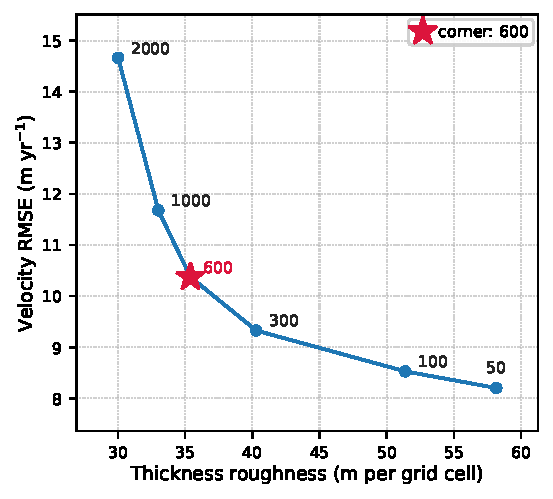
\includegraphics[width=0.5\linewidth]{figs/fig_da_lcurve.pdf}
  \caption{\DIFaddFL{Selecting the smoothness weight of the data assimilation, shown for Great
    Aletsch. Each point is one assimilation, labelled by its Tikhonov weight:
    stronger smoothing lowers the thickness roughness (horizontal axis) but worsens
    the fit to the observed surface velocity (vertical axis). The corner of the curve
    (star) is the point beyond which further smoothing buys little reduction in
    roughness for a rapidly rising misfit, and fixes the weight used thereafter. The
    same sequence of weights and the same corner-detection rule are applied to all
    three glaciers, returning 100 (Argenti\`ere), 600 (Great Aletsch) and 1000
    (Rh\^one).}}
  \label{fig:dalcurve}
\end{figure}


\DIFaddend The emulated flow regime is not set by the geometry alone: it also depends on two
scalar physical parameters, the basal-motion parameter $\tau_{\mathrm{ref}}$ and
the Arrhenius factor $A$. Here $\tau_{\mathrm{ref}}$ \DIFaddbegin \DIFadd{(in MPa) }\DIFaddend is the reference
basal shear stress in Weertman's sliding law \citep{weertman1957}---the shear stress sustaining a
reference basal speed of $100\,\mathrm{m\,yr^{-1}}$\DIFdelbegin \DIFdel{, in MPa---so }\DIFdelend \DIFaddbegin \DIFadd{---so }\DIFaddend that a smaller
$\tau_{\mathrm{ref}}$ corresponds
to easier sliding. Rather than invert these pointwise, we fix them beforehand by an
ensemble search: candidate $(\tau_{\mathrm{ref}}, A)$ pairs are drawn log-uniformly
from $[0.05, 2.0]\,\mathrm{MPa}$ and $[30, 200]\,\mathrm{MPa^{-3}\,yr^{-1}}$ by a
Tree-structured Parzen Estimator \citep[TPE;][]{bergstra2011}, as implemented in
Optuna \citep{akiba2019}, and each pair is passed
through the data assimilation; we retain the pair that minimises the
surface-velocity misfit, so the assimilation itself inverts the thickness $H$ alone.
We apply this identical procedure to all three glaciers, which keeps the pipeline
free of glacier-specific tuning. 

Data assimilation inverts the thickness at the \DIFdelbegin \DIFdel{start epoch $t_1$, which we
denote $H_{t_1}$}\DIFdelend \DIFaddbegin \DIFadd{epoch closest to the velocity
observations---the end epoch $t_2$ for all three glaciers studied here---which we
denote $H_{t_2}$}\DIFaddend . Finding the thickness fixes the bedrock,
\begin{equation}
  z_b(\mathbf{x}) = z_s^{\mathrm{obs}}(\mathbf{x}, t\DIFdelbegin \DIFdel{_1}\DIFdelend \DIFaddbegin \DIFadd{_2}\DIFaddend ) - H\DIFdelbegin \DIFdel{_{t_1}}\DIFdelend \DIFaddbegin \DIFadd{_{t_2}}\DIFaddend (\mathbf{x}),
  \label{eq:bed}
\end{equation}
which provides the substrate on which the transient run subsequently evolves\DIFdelbegin \DIFdel{.
}\DIFdelend \DIFaddbegin \DIFadd{: held
fixed, it also gives the thickness at the start epoch $t_1$ directly from the
observed $t_1$ DEM (Sect.~\ref{sec:inference}).
}\DIFaddend Only once the calibrated state matches the observed velocity
to within observational uncertainty do we accept it and proceed to the SMB
inversion.

\subsection{SMB inference by automatic differentiation}\label{sec:inference}

\paragraph{\DIFdelbegin \DIFdel{Observation }\DIFdelend \DIFaddbegin \DIFadd{Initial condition and }\DIFaddend target.}
With the dynamical state calibrated \DIFaddbegin \DIFadd{at $t_2$ }\DIFaddend (Sect.~\ref{sec:da}), the \DIFdelbegin \DIFdel{$smb$ }\DIFdelend \DIFaddbegin \DIFadd{SMB }\DIFaddend inversion
is driven by the geometry change between the two DEM epochs. The bedrock is already
fixed through Eq.~\eqref{eq:bed}; combining it with the observed \DIFdelbegin \DIFdel{end-of-window
}\DIFdelend \DIFaddbegin \DIFadd{start-of-window
}\DIFaddend surface DEM gives the \DIFdelbegin \DIFdel{target thickness }\DIFdelend \DIFaddbegin \DIFadd{thickness that initialises the forward run,
}\DIFaddend \begin{equation}
  H\DIFdelbegin \DIFdel{^{\mathrm{obs}}}\DIFdelend \DIFaddbegin \DIFadd{_{t_1}}\DIFaddend (\mathbf{x}\DIFdelbegin \DIFdel{, t_2}\DIFdelend ) = z_s^{\mathrm{obs}}(\mathbf{x}, t\DIFdelbegin \DIFdel{_2}\DIFdelend \DIFaddbegin \DIFadd{_1}\DIFaddend ) - z_b(\mathbf{x}).
  \DIFdelbegin %DIFDELCMD < \label{eq:hobs}
%DIFDELCMD < %%%
\DIFdelend \DIFaddbegin \label{eq:hinit}
\DIFaddend \end{equation}
\DIFdelbegin \DIFdel{The two surface DEMs $z_s^{\mathrm{obs}}(\cdot, t_1)$ and
$z_s^{\mathrm{obs}}(\cdot, t_2)$ are the glacier-specific two-epoch elevation models
of Sect.~\ref{sec:data}; their difference defines the geometry change the inversion
must reproduce}\DIFdelend \DIFaddbegin \DIFadd{By the same construction, combining the fixed bedrock with the observed
end-of-window surface DEM returns exactly the DA-calibrated thickness,
}\begin{equation}
  \DIFadd{H^{\mathrm{obs}}(\mathbf{x}, t_2) = z_s^{\mathrm{obs}}(\mathbf{x}, t_2) - z_b(\mathbf{x}) \equiv H_{t_2}(\mathbf{x}),
  \label{eq:hobs}
}\end{equation}
\DIFadd{which is therefore the target the forward run is fitted against: the data
assimilation's own calibrated state rather than an independent observation}\DIFaddend .
\paragraph{Forward model.}
With the \DIFdelbegin \DIFdel{calibrated }\DIFdelend \DIFaddbegin \DIFadd{derived }\DIFaddend thickness $H_{t_1}$ \DIFaddbegin \DIFadd{(Eq.~\ref{eq:hinit}) }\DIFaddend and the flow scalars
$(\tau_{\mathrm{ref}}, A)$ held fixed, the glacier is evolved from $t_1$ to $t_2$ by
integrating \eqref{eq:masscons} with an explicit forward-Euler scheme,
\begin{equation}
  H^{n+1} = \max\!\big(0,\; H^n + \Delta t^n [\,smb^n - \nabla\cdot\mathbf{q}^n\,]\big),
  \label{eq:euler}
\end{equation}
where the non-negativity projection prevents spurious negative thicknesses near the
margin. The integration starts from $H^0 = H_{t_1}$ and advances until the accumulated
time reaches $t_2$; the number of steps $N_t$ is therefore not prescribed but follows
from the step sizes selected along the way. Each step is limited by a
Courant--Friedrichs--Lewy condition,
\begin{equation}
  \Delta t^n = \min\!\Big(c_{\mathrm{cfl}}\,\Delta x \big/
  \max_\Omega\|\bar{\mathbf{u}}^n\|,\;\; \Delta t_{\max}\Big),
  \label{eq:cfl}
\end{equation}
with \DIFdelbegin \DIFdel{$c_{\mathrm{cfl}} = 0.2 < 1$ }\DIFdelend \DIFaddbegin \DIFadd{$c_{\mathrm{cfl}} = 0.2$ }\DIFaddend ensuring stability and
$\Delta t_{\max} = 1\,\mathrm{yr}$ capping the step where the ice is slow. The flux
divergence is evaluated on the staggered grid with a slope-limited scheme, which
suppresses spurious oscillations at the steep thickness gradients near the margin. At
every step the surface is updated as $z_s^n = z_b + H^n$ and $\bar{\mathbf{u}}$ is
recomputed by the emulator from the current $(H, z_s)$, so the flux divergence evolves
with the geometry rather than being held at its initial-snapshot value. Conventional
flux-divergence methods \citep{miles2021, kneib2024}, which we retain as a reference in
Sect.~\ref{sec:results}, instead evaluate $smb = \partial H/\partial t +
\nabla\cdot\mathbf{q}$ once from the calibrated state\DIFdelbegin \DIFdel{; because the divergence of a
flux built from two independently measured fields is itself dominated by small-scale
noise, such estimates require }\emph{\DIFdel{post hoc}} %DIFAUXCMD
\DIFdel{spatial smoothing}\DIFdelend .

\paragraph{SMB parametrisation.}
Rather than treat the $smb$ as an independent unknown at every grid cell, which would
leave the inversion severely underdetermined, we parametrise it as a one-dimensional
profile $smb(z)$, a function of surface elevation only.
This reflects the first-order elevation control on alpine $smb$ and collapses the unknown
from $\mathcal{O}(10^4)$ pixels to $N = \mathcal{O}(10)$ elevation bins, which
regularises the otherwise severely ill-posed inversion without site-specific
smoothing length scales or density assumptions. The profile is discretised on
uniformly spaced elevation bins, $200\,\mathrm{m}$ wide for all three glaciers, by the
values $\mathbf{m} = (m_1, \ldots, m_N)$, and
it is mapped to the two-dimensional source term in \eqref{eq:masscons} by
evaluating it at the current surface elevation,
$smb(\mathbf{x}, t) = smb(z_s(\mathbf{x}, t))$, with piecewise-linear interpolation
between bins (Fig.~\ref{fig:prof2field}). The parametrisation is deliberately minimal:
our aim is an $smb$ that explains the observed geometry change, not the resolution of
its fine spatial structure.

\begin{figure*}
  \centering
  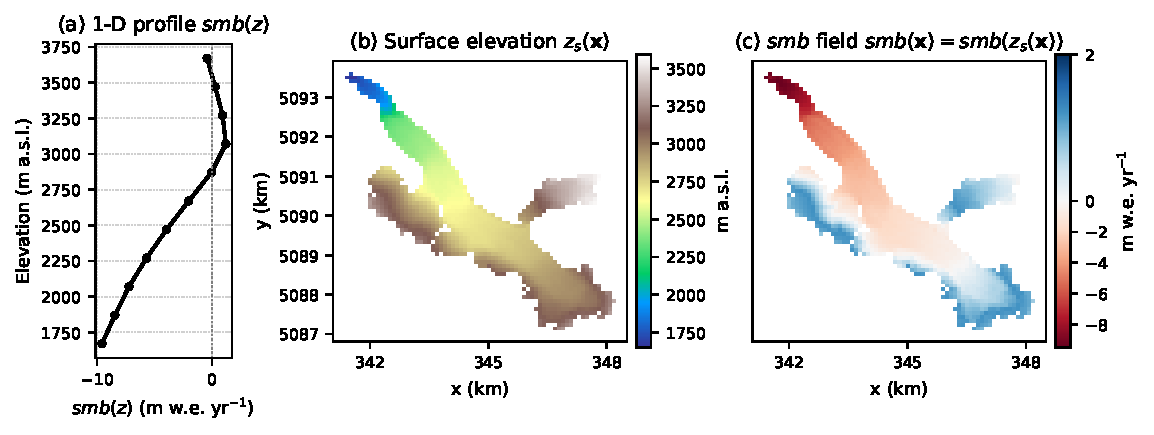
\includegraphics[width=\linewidth]{figs/fig_profile_to_field.pdf}
  \caption{Mapping the one-dimensional profile to the two-dimensional source term,
    $smb(\mathbf{x}) = smb(z_s(\mathbf{x}))$, on Argentière. (a)~The inferred
    elevation profile $smb(z)$; (b)~the surface elevation $z_s(\mathbf{x})$; and
    (c)~the resulting 2D $smb$ field, obtained by evaluating the profile at the surface
    elevation of every grid cell.}
  \label{fig:prof2field}
\end{figure*}

\paragraph{Inverse problem.}
We seek the smb profile $\mathbf{m}^\star$ that minimises the misfit between the
simulated end-of-window thickness $H^{\mathrm{sim}}(\cdot, t_2; \mathbf{m})$ and the
target $H^{\mathrm{obs}}(\cdot, t_2)$ from \eqref{eq:hobs}:
\begin{equation}
  \mathcal{J}(\mathbf{m}) =
  \sqrt{\frac{1}{|\Omega|}\sum_{\mathbf{x}\in\Omega}
    \big(H^{\mathrm{sim}} - H^{\mathrm{obs}}\big)^2}
  \;+\; \mathcal{R}(\mathbf{m}),
  \label{eq:cost}
\end{equation}
where the first term is the RMS geometry misfit and
$\mathcal{R}(\mathbf{m}) = \lambda \sum_i (m_{i-1} - 2m_i + m_{i+1})^2$ is a
Tikhonov smoothness penalty on the squared discrete curvature of the profile.
The weight $\lambda$ carries a direct physical reading: it sets how much the $smb$ may
change from one elevation bin to the next, and hence how strongly the recovered
gradient is smoothed \DIFaddbegin \DIFadd{(Fig \ref{fig:lambda})}\DIFaddend . We use \DIFdelbegin \DIFdel{$\lambda = 0.1$ throughout; the same value proved
optimal }\DIFdelend \DIFaddbegin \DIFadd{$\lambda = 0.05$ }\DIFaddend for all three glaciers \DIFdelbegin \DIFdel{, which suggests it may transfer to alpine glaciers
more generally. }\DIFdelend \DIFaddbegin \DIFadd{rather than
tuning it per site. Varying it over $0.01$--$0.5$ on Rhône moves the geometry misfit
by less than $5\,\%$ while the profile roughness falls by an order of magnitude
(Fig.~\ref{fig:lambda}a), and the recovered profile is insensitive through the centre
of that range: between $\lambda = 0.05$ and $0.1$ the equilibrium-line altitude is
unchanged and the stake RMSE differs by $0.01\,\mathrm{m\,w.e.\,yr^{-1}}$
(Fig.~\ref{fig:lambda}b). Only the extremes degrade the fit, the profile tracking
noise in the geometry change at $\lambda = 0.01$ and being over-smoothed at
$\lambda = 0.5$. }\DIFaddend The minimisation uses
L-BFGS \citep{liunocedal1989} with $M = 10$ correction pairs and a Hager--Zhang line
search; the low dimensionality of $\mathbf{m}$ makes the implicit Hessian
approximation accurate, and convergence is reached in $\mathcal{O}(10^2)$ function
evaluations.

\DIFaddbegin \begin{figure*}
  \centering
  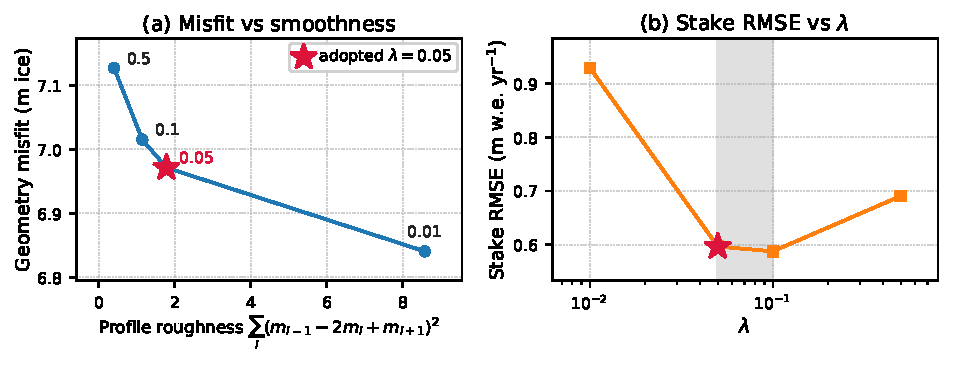
\includegraphics[width=0.8\linewidth]{figs/fig_lambda_lcurve.pdf}
  \caption{\DIFaddFL{Choice of the smoothness weight $\lambda$, shown for Rhône. Each point is
    one inversion, all sharing the same calibrated dynamical state so that only
    $\lambda$ varies. (a)~Stronger smoothing lowers the roughness of the profile at
    the cost of the geometry misfit. (b)~Stake RMSE against $\lambda$; the shaded
    band marks the range over which the recovered profile is effectively unchanged,
    and the fit degrades only at the extremes. The star is the adopted
    $\lambda = 0.05$.}}
  \label{fig:lambda}
\end{figure*}

\DIFaddend The gradient
$\nabla_{\mathbf{m}}\mathcal{J}$ is obtained by reverse-mode automatic
differentiation \citep{baydin2018} through the entire forward integration
\eqref{eq:masscons}--\eqref{eq:euler}: every operation in the forward map---the
emulator evaluation, the slope-limited divergence, the explicit Euler update and
the piecewise-linear elevation interpolation---is a differentiable TensorFlow
\citep{abadi2016} operation, so the chain rule applies uniformly across the forward
graph and the sensitivity of the end-of-window geometry to each bin value is
propagated exactly through every time step.

The principal cost is memory. Automatic differentiation must retain intermediate
quantities from the forward run in order to traverse it backwards, and a decade-long
integration exceeds the memory of a single GPU. We therefore use gradient
checkpointing \citep{griewank2000, chen2016}: instead of storing the internal
quantities of every step, we keep only the glacier state $(H, z_s)$ at the start of
each step and recompute that step's internals when the backward pass reaches it. The
saving is substantial because the emulator evaluation---by far the heaviest part of a
step---is never stored, only replayed; the price is one additional evaluation of each
step per gradient.
\DIFdelbegin %DIFDELCMD < 

%DIFDELCMD < %%%
\DIFdelend \section{Results}\label{sec:results}

We evaluate the method on three Alpine glaciers of contrasting size---Argentière,
Great Aletsch and Rhône---each processed through the same glacier-agnostic two-step
pipeline: the data assimilation inverts the ice thickness while the \DIFaddbegin \DIFadd{Arrhenius factor $A$ and the }\DIFaddend basal-motion
parameter $\tau_{\mathrm{ref}}$ \DIFdelbegin \DIFdel{is }\DIFdelend \DIFaddbegin \DIFadd{are }\DIFaddend fixed by an ensemble search to the scalar that
minimises the surface-velocity misfit, after which the $smb$ is inferred. No
per-glacier retuning of the regularisation, optimiser or parametrisation is applied,
and none of the three uses a thickness survey. Argentière additionally carries the
state-of-the-art distributed reconstruction of \citet{kneib2024}, against which we
compare our velocity-only result directly.


\subsection{Calibrated ice-dynamics states}\label{sec:calib}

For every glacier the data assimilation converges within $\mathcal{O}(10^2)$ L-BFGS
iterations to a thickness field whose modelled surface velocity matches the
observations to a root-mean-square residual of \DIFdelbegin \DIFdel{a few $\mathrm{m\,yr^{-1}}$}\DIFdelend \DIFaddbegin \DIFadd{order $1$--$10\,\mathrm{m\,yr^{-1}}$}\DIFaddend ---\DIFdelbegin \DIFdel{$2.4$ }\DIFdelend \DIFaddbegin \DIFadd{$1.0$ }\DIFaddend on
Argentière, \DIFdelbegin \DIFdel{$11$ }\DIFdelend \DIFaddbegin \DIFadd{$10.3$ }\DIFaddend on Great Aletsch and \DIFdelbegin \DIFdel{$6.8$ }\DIFdelend \DIFaddbegin \DIFadd{$7.8$ }\DIFaddend on Rhône at the adopted
\DIFaddbegin \DIFadd{(}\DIFaddend $\tau_{\mathrm{ref}}$\DIFaddbegin \DIFadd{, A)}\DIFaddend ---one to two orders of magnitude
below typical trunk velocities (locally exceeding
$100$--$150\,\mathrm{m\,yr^{-1}}$). The calibrated state fixes the bedrock through
Eq.~\eqref{eq:bed}\DIFdelbegin \DIFdel{and provides the starting }\DIFdelend \DIFaddbegin \DIFadd{, from which the start-epoch }\DIFaddend geometry $H_{t_1}$ \DIFdelbegin \DIFdel{for }\DIFdelend \DIFaddbegin \DIFadd{is derived to
initialise }\DIFaddend the transient forward run (Sect.~\ref{sec:inference}).

Figure~\ref{fig:da-state} shows the calibrated state on Argentière: the recovered
ice-thickness field (a), and the close match between the observed (b) and modelled
(c) surface speed, whose differences are small and spatially unstructured.

\begin{figure*}
  \centering
  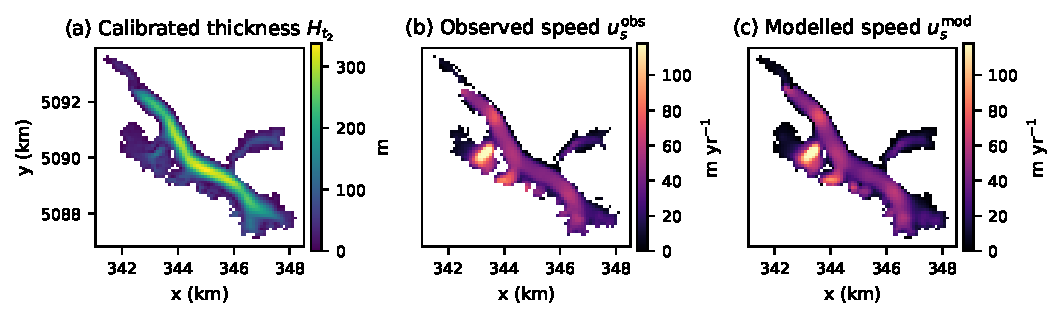
\includegraphics[width=\linewidth]{figs/fig_da_state.pdf}
  \caption{Calibrated data-assimilation state on Argentière at the \DIFdelbeginFL \DIFdelFL{start }\DIFdelendFL \DIFaddbeginFL \DIFaddFL{calibration
    }\DIFaddendFL epoch \DIFaddbeginFL \DIFaddFL{$t_2$}\DIFaddendFL , for the adopted velocity-only run
    (\DIFdelbeginFL \DIFdelFL{$\tau_{\mathrm{ref}}=0.27\,\mathrm{MPa}$}\DIFdelendFL \DIFaddbeginFL \DIFaddFL{$\tau_{\mathrm{ref}}=0.199\,\mathrm{MPa}$}\DIFaddendFL ).
    (a)~Calibrated ice thickness \DIFdelbeginFL \DIFdelFL{$H_{t_1}$}\DIFdelendFL \DIFaddbeginFL \DIFaddFL{$H_{t_2}$}\DIFaddendFL ; (b)~observed surface speed
    $u_s^{\mathrm{obs}}$ \citep{millan2022}; (c)~modelled surface speed
    $u_s^{\mathrm{mod}}$, in close agreement with the observations.}
  \label{fig:da-state}
\end{figure*}

As a final check \DIFdelbegin \DIFdel{, we confirm }\DIFdelend \DIFaddbegin \DIFadd{on }\DIFaddend the calibrated state \DIFdelbegin \DIFdel{is free of the initialisation
shock of Sect.~\ref{sec:overview}: integrated }\DIFdelend \DIFaddbegin \DIFadd{itself, Appendix~\ref{app:equilibrium}
integrates both candidate starting states on Argentière ($H_{t_1}$, $H_{t_2}$)
}\DIFaddend forward for one year under zero $smb$\DIFdelbegin \DIFdel{,
it produces no spurious thickness drift , so }\DIFdelend \DIFaddbegin \DIFadd{: both drift with a near-zero mean
($-0.3$ and $-0.1\,\mathrm{m}$), so neither is spontaneously gaining or losing
mass under the calibrated dynamics---confirming }\DIFaddend the \DIFdelbegin \DIFdel{glacier is in mechanical equilibrium
and any subsequent geometry change is attributable to the prescribed }\DIFdelend \DIFaddbegin \DIFadd{fixed-substrate assumption of
Sect.~\ref{sec:overview} is not masking a systematic bias that the }\DIFaddend $smb$ \DIFdelbegin \DIFdel{rather
than to residual model imbalance}\DIFdelend \DIFaddbegin \DIFadd{inversion
would otherwise have to absorb}\DIFaddend .

\subsection{Inferred SMB and validation}\label{sec:inferred}

Holding the calibrated state (\DIFdelbegin \DIFdel{$H_{t_1}$, }\DIFdelend \DIFaddbegin \DIFadd{the bedrock fixed via $H_{t_2}$, and }\DIFaddend $\tau_{\mathrm{ref}}$, $A$) \DIFaddbegin \DIFadd{and the derived start-epoch thickness $H_{t_1}$ }\DIFaddend fixed, we run the
transient forward simulation over each glacier's window and invert for the
elevation-resolved $smb$ profile $smb(z)$ that minimises the geometry-misfit cost
(Eq.~\ref{eq:cost}). On all three glaciers the retrieved profile increases
monotonically across the full altitudinal range, from strongly negative values at
the tongue to a positive accumulation regime in the upper basin.

On Argentière (2012--2021) the profile reproduces the observed altitudinal pattern
of the GLACIOCLIM stakes with a root-mean-square error of
\DIFdelbegin \DIFdel{$0.65\,\mathrm{m\,w.e.\,yr^{-1}}$ }\DIFdelend \DIFaddbegin \DIFadd{$0.40\,\mathrm{m\,w.e.\,yr^{-1}}$ }\DIFaddend (Fig.~\ref{fig:smb-continuity}a,
Table~\ref{tab:rmse}). This is obtained with the generic velocity-only
pipeline---no thickness survey, no per-glacier tuning, no \emph{post hoc}
smoothing---yet it \DIFdelbegin \DIFdel{is on par with the best physically-based }\DIFdelend \DIFaddbegin \DIFadd{surpasses the best physically based }\DIFaddend reconstructions of
\citet{kneib2024} on the same stakes, whose \DIFaddbegin \DIFadd{flux-gate F2019 estimate gives $0.50$
and whose }\DIFaddend SIA and IGM-distributed approaches give $0.67$ and
$0.85\,\mathrm{m\,w.e.\,yr^{-1}}$\DIFdelbegin \DIFdel{and whose flux-gate F2019 estimate
gives $0.50$}\DIFdelend , all of which additionally require ice-thickness
data. \DIFdelbegin \DIFdel{Argentière is also covered by accurate GPR thickness soundings; repeating the
experiment with them---inverting $\tau_{\mathrm{ref}}$ as a spatial field---lowers
the error further and surpasses every published reconstruction on this site, as
detailed in Appendix~A1. }\DIFdelend Because the inversion variable is one-dimensional,
horizontal heterogeneity within an elevation band---notably the avalanche-fed
accumulation hotspots reported by \citet{kneib2024}---is not resolved; this
deliberate trade-off, which buys a tuning-free and transferable inversion, is taken
up in Sect.~\ref{sec:discussion}.

\begin{table}
    \centering
    \caption{Validation of the inferred SMB against the GLACIOCLIM stake network on
    Argentière Glacier (main trunk + Améthystes tributary) over 2012--2021. The
    three baselines are the modelling approaches of \citet{kneib2024}, evaluated
    against the same stakes; all three use ice-thickness data, whereas our result
    uses surface velocity only.\DIFdelbeginFL \DIFdelFL{The GPR-assisted field inversion, which improves
    further on these, is reported in Appendix~A1.}\DIFdelendFL }
    \label{tab:rmse}
    \begin{tabular}{lc}
        \hline
        Method & RMSE [m\,w.e.\,yr$^{-1}$] \\
        \hline
        F2019 \citep{kneib2024}                       & 0.50 \\
        SIA \citep{kneib2024}                          & 0.67 \\
        IGM-distributed \citep{kneib2024}              & 0.85 \\
        \textbf{Ours (velocity only, scalar $\tau_{\mathrm{ref}}$)} & \textbf{\DIFdelbeginFL \DIFdelFL{0.65}\DIFdelendFL \DIFaddbeginFL \DIFaddFL{0.40}\DIFaddendFL } \\
        \hline
    \end{tabular}
\end{table}

The same pipeline, applied without modification to Great Aletsch (2009--2017) and
Rhône (2007--2016), yields equally smooth, monotonic profiles that reproduce the
independent stake averages---two continuous-record locations on Aletsch and five on
Rhône (Sect.~\ref{sec:data})---with root-mean-square errors of \DIFdelbegin \DIFdel{$0.61$ and
$0.32\,\mathrm{m\,w.e.\,yr^{-1}}$ }\DIFdelend \DIFaddbegin \DIFadd{$0.52$ and
$0.60\,\mathrm{m\,w.e.\,yr^{-1}}$ }\DIFaddend (Fig.~\ref{fig:smb-continuity}b,c). 
\DIFdelbegin \DIFdel{These are on par with the Argentière result despite the absence of }\DIFdelend \DIFaddbegin \DIFadd{This fit without }\DIFaddend any thickness constraint \DIFdelbegin \DIFdel{, which we read }\DIFdelend \DIFaddbegin \DIFadd{reads }\DIFaddend less as a
coincidence than as evidence that the velocity-calibrated dynamical
state carries the elevation structure of the SMB; whether the robustness holds
across a larger and more varied sample than three \DIFdelbegin \DIFdel{large }\DIFdelend \DIFaddbegin \DIFadd{well-monitored }\DIFaddend glaciers is an open question
we return to in Sect.~\ref{sec:discussion}.

\begin{figure*}
  \centering
  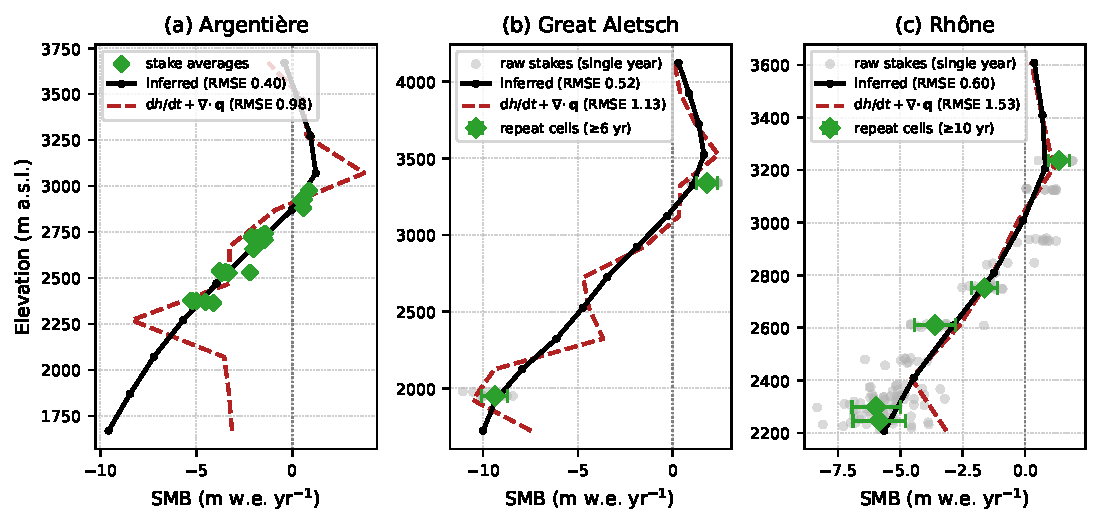
\includegraphics[width=\linewidth]{figs/fig_continuity_3panel.pdf}
  \caption{Inferred SMB profile (black) for (a)~Argentière, (b)~Great Aletsch and
    (c)~Rhône, compared against in situ stake measurements and against the continuity
    estimate $\mathrm{d}h/\mathrm{d}t + \nabla\!\cdot\mathbf{q}$ (dashed) obtained with
    the \emph{stationary} data-assimilation flux divergence. Green diamonds are the
    continuous-record stake averages ($\pm$ interannual standard deviation), the
    validation targets (faint grey dots on Aletsch and Rhône are the raw single-year
    readings). The inferred profile tracks the averages across the whole elevation
    range (\DIFdelbeginFL \DIFdelFL{$\mathrm{RMSE}=0.65$}\DIFdelendFL \DIFaddbeginFL \DIFaddFL{$\mathrm{RMSE}=0.40$}\DIFaddendFL , \DIFdelbeginFL \DIFdelFL{$0.61$ }\DIFdelendFL \DIFaddbeginFL \DIFaddFL{$0.52$ }\DIFaddendFL and \DIFdelbeginFL \DIFdelFL{$0.32\,\mathrm{m\,w.e.\,yr^{-1}}$}\DIFdelendFL \DIFaddbeginFL \DIFaddFL{$0.60\,\mathrm{m\,w.e.\,yr^{-1}}$}\DIFaddendFL ),
    whereas the stationary-flux estimate departs strongly in the ablation zone
    (\DIFdelbeginFL \DIFdelFL{$2.14$}\DIFdelendFL \DIFaddbeginFL \DIFaddFL{$0.98$}\DIFaddendFL , \DIFdelbeginFL \DIFdelFL{$1.59$ }\DIFdelendFL \DIFaddbeginFL \DIFaddFL{$1.13$ }\DIFaddendFL and \DIFdelbeginFL \DIFdelFL{$1.63$}\DIFdelendFL \DIFaddbeginFL \DIFaddFL{$1.53$}\DIFaddendFL ).}
  \label{fig:smb-continuity}
\end{figure*}

Figure~\ref{fig:smb-continuity} makes concrete the
mass-conservation argument of Sect.~\ref{sec:sota}. The dashed curve is the SMB the
continuity equation yields when the flux divergence is taken as stationary, exactly
as in flux-divergence inversions. On every glacier this estimate is markedly noisier
than the inferred profile and diverges in the ablation zone, where the stationary
divergence is least representative, raising the stake RMSE to \DIFdelbegin \DIFdel{$2.14$ }\DIFdelend \DIFaddbegin \DIFadd{$0.98$ }\DIFaddend (Argentière),
\DIFdelbegin \DIFdel{$1.59$ }\DIFdelend \DIFaddbegin \DIFadd{$1.13$ }\DIFaddend (Aletsch) and \DIFdelbegin \DIFdel{$1.63\,\mathrm{m\,w.e.\,yr^{-1}}$ }\DIFdelend \DIFaddbegin \DIFadd{$1.53\,\mathrm{m\,w.e.\,yr^{-1}}$ }\DIFaddend (Rhône)---a factor of \DIFdelbegin \DIFdel{$2.6$ to
$5$ }\DIFdelend \DIFaddbegin \DIFadd{$2.2$ to
$2.5$ }\DIFaddend worse than our transient inversion. Because our forward model integrates the
mass-conservation law directly and recomputes the flux divergence from the evolving
geometry at every step, the inferred profile requires no spatial smoothing and
remains mass-consistent throughout.

\subsection{Sensitivity to the basal-motion parameter}\label{sec:sensitivity}

The basal-motion parameter $\tau_{\mathrm{ref}}$ is the dynamical quantity least
constrained on a glacier without thickness or stake data, where its value rests on
the surface-velocity misfit (\emph{velsurf}) alone. It is also intrinsically hard to
separate from the ice thickness: a more slippery bed (smaller $\tau_{\mathrm{ref}}$)
inferred together with thinner ice reproduces almost the same surface
velocity---and hence the same ice flux---as a stiffer bed carrying thicker ice, so
many $(\tau_{\mathrm{ref}}, H)$ pairs fit the observations nearly equally well. For
the $smb$ inversion this ambiguity is not fatal, because what drives the geometry
change is not the pair itself but the flux divergence $\nabla\!\cdot\mathbf{q}$ it
produces. To see how the residual freedom in $\tau_{\mathrm{ref}}$ propagates into the
inferred $smb$, we repeated the $smb$ inversion across a wide range of
$\tau_{\mathrm{ref}}$ on all three glaciers (Fig.~\ref{fig:sens}), using the
independent stake RMSE as ground truth against \emph{velsurf}, the only selector
available operationally.

\begin{figure*}
  \centering
  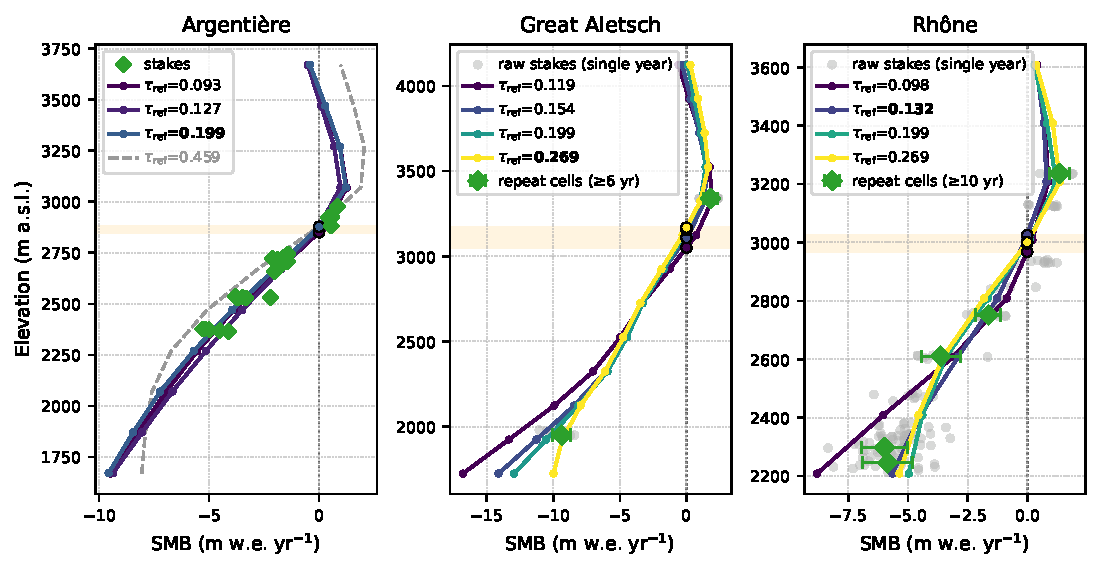
\includegraphics[width=\linewidth]{figs/sens_slidingco_3panel.pdf}
  \caption{Inferred SMB profiles across a range of the basal-motion parameter
    $\tau_{\mathrm{ref}}$ for (a)~Argentière, (b)~Great Aletsch and (c)~Rhône;
    colour encodes $\tau_{\mathrm{ref}}$ and the adopted profile is drawn bold.
    Within the low-velocity-misfit basin the profiles coincide in the accumulation
    area and diverge only at the ablation tongue, so the residual uncertainty in
    $\tau_{\mathrm{ref}}$ translates into an equilibrium-line-altitude band (shaded)
    rather than a whole-profile bias; the runs the velocity misfit rejects (dashed)
    depart most strongly.}
  \label{fig:sens}
\end{figure*}

Two features stand out. First, \emph{velsurf} reliably rejects the strongly biased
runs: the profiles that depart most from the stakes are also those with the worst
velocity misfit (Fig.~\ref{fig:sens}). \DIFdelbegin \DIFdel{Pooled across the three glaciers}\DIFdelend \DIFaddbegin \DIFadd{On each glacier}\DIFaddend , higher velocity misfit goes
with higher stake error (Fig.~\ref{fig:corr}; Pearson \DIFdelbegin \DIFdel{$r=0.69$, $p<10^{-2}$}\DIFdelend \DIFaddbegin \DIFadd{$r=0.99$, Spearman
$\rho=0.83$ on Argentière; $r=0.72$, $\rho=0.38$ on Aletsch; $r=0.81$, $\rho=0.71$ on
Rhône}\DIFaddend ). Second, once the\DIFdelbegin \DIFdel{se}\DIFdelend  high-misfit runs are removed, the surviving
low-\emph{velsurf} runs no longer map one-to-one onto stake error: because a wide
range of $(\tau_{\mathrm{ref}}, H)$ pairs share nearly the same flux, velocity cannot
single out one value of $\tau_{\mathrm{ref}}$, and on Rhône the stake RMSE even varies
non-monotonically among them (\DIFdelbegin \DIFdel{$0.32$}\DIFdelend \DIFaddbegin \DIFadd{$0.60$}\DIFaddend --\DIFdelbegin \DIFdel{$1.25\,\mathrm{m\,w.e.\,yr^{-1}}$}\DIFdelend \DIFaddbegin \DIFadd{$1.34\,\mathrm{m\,w.e.\,yr^{-1}}$}\DIFaddend ). Crucially,
this residual freedom is confined to the ablation zone: across the low-misfit runs
the accumulation-area profile is essentially unchanged, and only the tongue
$smb$---and with it the equilibrium-line altitude---shifts from run to run
(Fig.~\ref{fig:sens}).

\begin{figure}
  \centering
  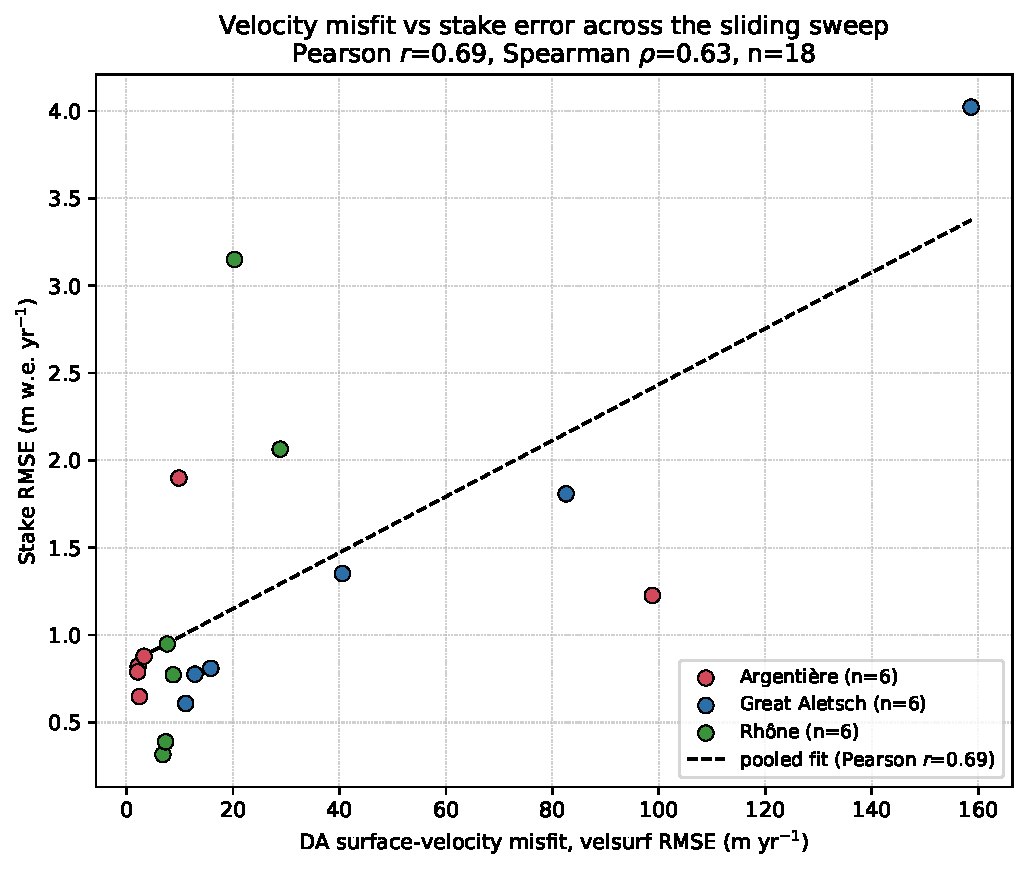
\includegraphics[width=0.6\linewidth]{figs/velsurf_vs_stake_rmse.pdf}
  \caption{Data-assimilation surface-velocity misfit (\emph{velsurf} RMSE) against
    the independent stake RMSE \DIFdelbeginFL \DIFdelFL{, pooled over }\DIFdelendFL \DIFaddbeginFL \DIFaddFL{across }\DIFaddendFL the $\tau_{\mathrm{ref}}$ sweep\DIFdelbeginFL \DIFdelFL{(six
    runs per glacier}\DIFdelendFL , \DIFdelbeginFL \DIFdelFL{all three glaciers)}\DIFdelendFL \DIFaddbeginFL \DIFaddFL{shown
    separately for each glacier}\DIFaddendFL . Higher velocity misfit is associated with higher
    stake error \DIFaddbeginFL \DIFaddFL{on all three }\DIFaddendFL (Pearson \DIFdelbeginFL \DIFdelFL{$r=0.69$}\DIFdelendFL \DIFaddbeginFL \DIFaddFL{$r=0.99$}\DIFaddendFL , \DIFaddbeginFL \DIFaddFL{$0.72$ and $0.81$; }\DIFaddendFL Spearman
    \DIFdelbeginFL \DIFdelFL{$\rho=0.63$}\DIFdelendFL \DIFaddbeginFL \DIFaddFL{$\rho=0.83$, $0.38$ and $0.71$, for Argentière, Aletsch and Rhône respectively}\DIFaddendFL ),
    so the velocity misfit---the only selector available without stakes---carries
    usable information about the accuracy of the inferred SMB.}
  \label{fig:corr}
\end{figure}

The practical consequence is that the method does not deliver a single ``best''
profile but a family of low-\emph{velsurf} solutions that converge to the same
accumulation-area gradient and fan out only at the tongue
(Fig.~\ref{fig:sens}, Fig.~\ref{fig:corr}). For a stake-free glacier this family is
the result: the low-misfit runs together define an $smb$ and equilibrium-line
uncertainty band---narrow in the accumulation area, widening towards the tongue. How
this band behaves at regional scale, and how it might be tightened, we take up in
Sect.~\ref{sec:discussion}.

\section{Discussion}\label{sec:discussion}

Separating surface mass balance from dynamic thinning in an observed
surface-elevation change is a notoriously ill-posed problem, yet it is exactly what
deriving SMB from remote sensing demands. We have addressed it with a transient,
differentiable inversion: a state-of-the-art assimilation of surface ice speed fixes
the dynamical state, and a novel automatic-differentiation scheme then inverts the
multi-temporal geometry change for the elevation-resolved SMB. On three Alpine
glaciers of contrasting size the method reproduces the in situ stake balances to
root-mean-square errors of \DIFdelbegin \DIFdel{$0.65$ }\DIFdelend \DIFaddbegin \DIFadd{$0.40$ }\DIFaddend (Argentière), \DIFdelbegin \DIFdel{$0.61$ }\DIFdelend \DIFaddbegin \DIFadd{$0.52$ }\DIFaddend (Great Aletsch) and
\DIFdelbegin \DIFdel{$0.32\,\mathrm{m\,w.e.\,yr^{-1}}$ }\DIFdelend \DIFaddbegin \DIFadd{$0.60\,\mathrm{m\,w.e.\,yr^{-1}}$ }\DIFaddend (Rhône), \DIFdelbegin \DIFdel{on par with the best physically-based
reconstructions }\DIFdelend \DIFaddbegin \DIFadd{surpassing the best physically based
reconstruction }\DIFaddend of \citet{kneib2024} on the same Argentière stakes \DIFdelbegin \DIFdel{and, where GPR
thickness is assimilated, surpassing them (Appendix~A1)}\DIFdelend \DIFaddbegin \DIFadd{with surface
velocity alone}\DIFaddend . Two features set the approach apart from that state of the art.
First, the flux divergence is recomputed from the evolving geometry at every time step
rather than held at a single stationary snapshot\DIFdelbegin \DIFdel{, }\DIFdelend \DIFaddbegin \DIFadd{. A stationary estimate evaluates
$\nabla\!\cdot\mathbf{q}$ once, on the geometry of a single epoch, and applies it to an
elevation change averaged over a decade---a decade over which the glacier thins, slows
and changes its flux. Integrating the mass-conservation equation forward removes that
assumption rather than correcting for it, }\DIFaddend so the inferred SMB is dynamically consistent
\DIFdelbegin \DIFdel{and avoids the ablation-zone bias that makes stationary-flux estimates a
factor of two to five worse }\DIFdelend \DIFaddbegin \DIFadd{across the whole window; }\DIFaddend against the same stakes\DIFdelbegin \DIFdel{.
}\DIFdelend \DIFaddbegin \DIFadd{, the stationary-flux estimate is
markedly worse on all three glaciers (Sect.~\ref{sec:results}).
}

\DIFaddend Second, the inversion needs only surface velocity---no
ice-thickness survey and no per-glacier tuning---and proved largely insensitive to
the rate factor $A$, so a single glacier-independent pipeline transfers across all
three sites. \DIFaddbegin \DIFadd{Beyond validating the inversion, the recovered $smb(z)$ is the quantity
mass-balance models are calibrated against: an elevation-resolved balance over a known
period is what a temperature-index or energy-balance model must reproduce before it can
be driven forward under a climate scenario. Inferring it from geometry alone therefore
offers a route to constraining such models---and with them, projections of glacier
change and meltwater supply---on the great majority of glaciers that carry no stake
record.
}\DIFaddend 

The clearest methodological gain is in how mass conservation is enforced.
Flux-divergence inversions form the SMB by differentiating the observed
thickness--velocity flux and combining it with the elevation-change field; because
that divergence is the spatial derivative of a product of two noisy fields, it must
be smoothed before use, and the smoothing---as \DIFaddbegin \DIFadd{\mbox{%DIFAUXCMD
\citet{miles2021} }\hskip0pt%DIFAUXCMD
and }\DIFaddend \citet{kneib2024}
document---breaks
the very mass-conservation constraint the method rests on, leaving a spurious
glacier-wide flux-divergence residual of order $0.1$--$0.7\,\mathrm{m\,yr^{-1}}$ that
they close by redistributing the excess or deficit uniformly across the glacier. Such
a homogeneous redistribution is a pragmatic fix rather than a physical statement: it
spreads a computational residual over cells that did not produce it. Our formulation
removes the need for either step. Because we integrate the mass-conservation equation
forward and evaluate the flux divergence on the modelled geometry with a
conservative, slope-limited scheme, mass is conserved by construction at every step;
the inferred SMB field requires no post-hoc smoothing and no ad-hoc redistribution,
and the divergence it implies is guaranteed consistent with the simulated geometry
change.

The \DIFaddbegin \DIFadd{contrast is visible in our own runs. The flux divergence implied by the calibrated
assimilation state is markedly rougher than the thickness field it derives from---
grid-scale structure carries three to four times the share of its variance---because
differentiating a product of two fields amplifies exactly the wavelengths the
assimilation constrains least. Integrating forward damps it: the flux is diffusive in
thickness, so by the end of the window the modelled divergence is smooth and spatially
coherent where the assimilated one was speckled. The filtering that flux-divergence
methods must impose externally is here a consequence of the ice dynamics rather than a
step applied afterwards.
}

\DIFadd{The }\DIFaddend method's principal limitation is its one-dimensional parametrisation: horizontal
variability within an elevation band---such as the avalanche-fed accumulation
hotspots resolved by \citet{kneib2024}---is deliberately not recovered. This buys a
transferable, tuning-free inversion and is not intrinsic to the scheme, which admits
richer descriptions (an aspect or debris-cover dependence, say) wherever the data
warrant them. A second limitation is the thickness--sliding ambiguity of
Sect.~\ref{sec:sensitivity}: surface velocity constrains the basal-motion parameter
only to a band, and the resulting freedom, negligible in the accumulation area, opens
into an equilibrium-line spread at the tongue. Two further dependencies are shared
with flux-based methods. Accuracy is ultimately set by the input velocity and DEMs:
\citet{kneib2024} find that substituting the coarser global velocity mosaic of
\citet{millan2022} into their reconstruction degrades the stake agreement to
$\sim$1.2--1.3$\,\mathrm{m\,w.e.\,yr^{-1}}$, so the velocity field can itself become
limiting---that our transient inversion attains \DIFdelbegin \DIFdel{$0.32$}\DIFdelend \DIFaddbegin \DIFadd{$0.40$}\DIFaddend --\DIFdelbegin \DIFdel{$0.65\,\mathrm{m\,w.e.\,yr^{-1}}$
}\DIFdelend \DIFaddbegin \DIFadd{$0.60\,\mathrm{m\,w.e.\,yr^{-1}}$
}\DIFaddend using precisely that global product is encouraging, but its robustness to velocity
error should not be overstated. Finally, like all geodetic estimates the method
converts a volume change to a mass balance under an assumed ice density and neglects
evolving firn compaction; where the firn column is thick or densifying, this
introduces a systematic offset.

Taken together, these properties point towards regional-scale application. Because the
pipeline requires no thickness survey, no stake calibration and no site-specific
tuning, it can in principle be applied wherever multi-temporal DEMs and a
surface-velocity field exist---and both are approaching near-global coverage, through
the elevation-change archive of \citet{hugonnet2021} and expanding velocity products
\citep{millan2022}. Its accuracy will track that of these inputs\DIFdelbegin \DIFdel{, so the highest
fidelity will come }\DIFdelend \DIFaddbegin \DIFadd{: substituting that
$\mathrm{d}h/\mathrm{d}t$ product for the dedicated DEM pair on
Rhône raises the stake error to $0.77\,\mathrm{m\,w.e.\,yr^{-1}}$ (from $0.60$),
while still
recovering the full altitudinal structure and remaining far better than the
stationary-flux estimate (Appendix~\ref{app:hugonnet}). The highest fidelity therefore
still comes }\DIFaddend from dedicated high-resolution DEMs\DIFdelbegin \DIFdel{; but the }\DIFdelend \DIFaddbegin \DIFadd{, but the method degrades gracefully
rather than failing where only near-global data exist; and the }\DIFaddend tuning-free character
makes a continuous, distributed SMB inversion over many glaciers a realistic next
step. Whether the robustness shown here on three \DIFdelbegin \DIFdel{large, }\DIFdelend well-monitored \DIFaddbegin \DIFadd{Alpine }\DIFaddend glaciers
persists across the smaller and more varied population that dominates regional water
resources is the key open question, and the natural direction for future work.

\section{Conclusions}\label{sec:conclusions}

We have presented a transient, differentiable inversion that recovers the distributed
surface mass balance of a glacier from two surface DEMs and a single surface-velocity
field, without ice-thickness measurements or per-glacier tuning. Surface velocity is
assimilated to fix a dynamically consistent state, and the mass-conservation equation
is then integrated forward with automatic differentiation to infer the
elevation-resolved SMB whose modelled geometry change best matches observation.
Applied through one glacier-independent pipeline to three Alpine glaciers of
contrasting size, the method reproduces in situ stake balances to
\DIFdelbegin \DIFdel{$0.32$}\DIFdelend \DIFaddbegin \DIFadd{$0.40$}\DIFaddend --\DIFdelbegin \DIFdel{$0.65\,\mathrm{m\,w.e.\,yr^{-1}}$---on par with, and where GPR thickness is
available surpassing, }\DIFdelend \DIFaddbegin \DIFadd{$0.60\,\mathrm{m\,w.e.\,yr^{-1}}$---surpassing }\DIFaddend the state-of-the-art
reconstruction of \citet{kneib2024} \DIFdelbegin \DIFdel{---and
}\DIFdelend \DIFaddbegin \DIFadd{on Argentière with surface velocity alone---and
}\DIFaddend a factor of \DIFdelbegin \DIFdel{two to five }\DIFdelend \DIFaddbegin \DIFadd{roughly two to two-and-a-half }\DIFaddend better than the
stationary-flux estimates it replaces.

The central advance is that mass conservation is enforced by construction: because the
flux divergence is recomputed from the evolving geometry at every step, the inferred
SMB needs neither the post-hoc smoothing nor the ad-hoc mass redistribution that
flux-divergence methods require, and stays dynamically consistent over the whole
observation window. Its accuracy is limited chiefly by the input velocity and DEMs and
by the one-dimensional elevation parametrisation, which trades sub-band spatial detail
for transferability. Because the method needs no calibration data beyond fields that
are approaching near-global coverage, it opens a realistic path towards continuous,
regional-scale SMB inversion; establishing its robustness across the smaller and more
varied glacier population that dominates regional water resources is the natural next
step.

%\newpage
\appendix
\section{Appendix}

\DIFdelbegin \subsection{\DIFdel{GPR-assisted basal-motion-field inversion on Argentière}}%DIFAUXCMD
\addtocounter{subsection}{-1}%DIFAUXCMD
%DIFDELCMD < \label{app:gpr}
%DIFDELCMD < 

%DIFDELCMD < %%%
\DIFdel{The main analysis fixes the basal-motion parameter $\tau_{\mathrm{ref}}$ to a single
scalar, so that all three glaciers are treated identically and no thickness survey is
required. Where dense auxiliary data }\emph{\DIFdel{do}} %DIFAUXCMD
\DIFdel{exist, however, the same differentiable
framework can exploit them to sharpen the dynamical state. Argentière is covered by
repeated ground-penetrating-radar (GPR) soundings of ice thickness
\mbox{%DIFAUXCMD
\citep{rabatel2018}}\hskip0pt%DIFAUXCMD
; here we show that assimilating them, and relaxing
$\tau_{\mathrm{ref}}$ from a scalar into a spatial field $\tau_{\mathrm{ref}}(\mathbf{x})$
inverted jointly with the thickness, further improves the fit and surpasses the state
of the art.
}%DIFDELCMD < 

%DIFDELCMD < %%%
\DIFdel{The GPR soundings supply an independent thickness constraint (the second term of
Eq.~\ref{eq:da}, over the survey footprint $\Omega_{\mathrm{thk}}$) that makes the
joint inversion identifiable. The data assimilation then retrieves both the
ice-thickness field $H_{t_1}$ and the basal-motion field
$\tau_{\mathrm{ref}}(\mathbf{x})$ that together reproduce the observed surface
velocity and the GPR transects, converging within $10^2$ L-BFGS iterations
(Fig.~A1). Modelled velocities match the observations to a
root-mean-square residual of $3\,\mathrm{m\,yr^{-1}}$, and the calibrated thickness
departs from the GPR transects by RMS $=12\,\mathrm{m}$ (bias $-9\,\mathrm{m}$), of
the order of the GPR uncertainty itself. The recovered sliding field shows the
physically expected structure---enhanced along the central flowline and reduced near
the lateral margins---consistent with the finding of \mbox{%DIFAUXCMD
\citet{kneib2024} }\hskip0pt%DIFAUXCMD
that spatial
variability in $\tau_{\mathrm{ref}}$ helps explain the observed surface velocities.
}%DIFDELCMD < 

%DIFDELCMD < \begin{figure*}
%DIFDELCMD <   \centering
%DIFDELCMD <   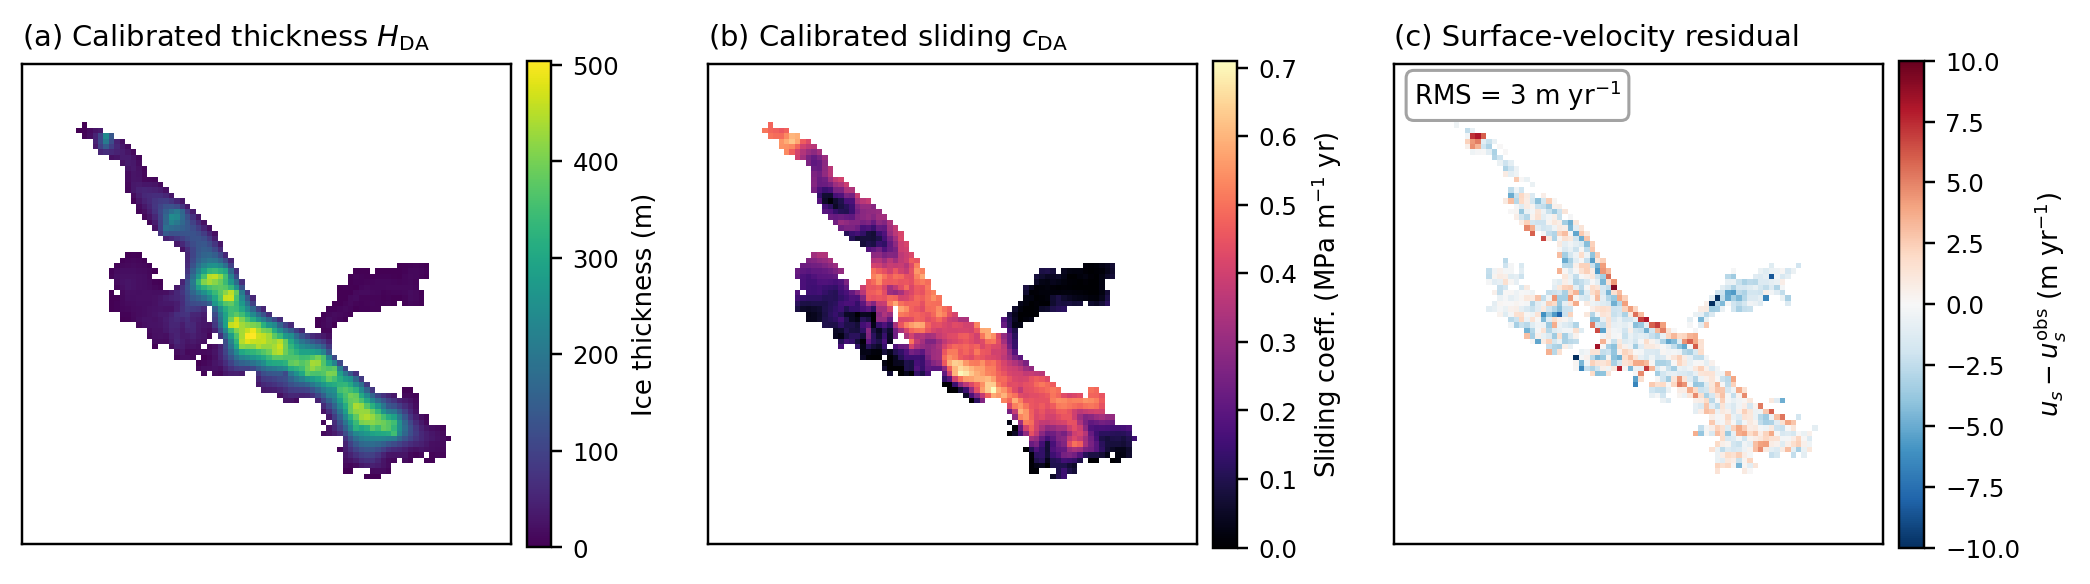
\includegraphics[width=\linewidth]{figs/argentiere_da_panel.png}
%DIFDELCMD <   %%%
%DIFDELCMD < \caption{%
{%DIFAUXCMD
\DIFdelFL{GPR-assisted data-assimilation state on Argentière Glacier at the start
    epoch. (a)~Calibrated ice thickness $H_{t_1}$ and (b)~calibrated basal-motion
    field $\tau_{\mathrm{ref}}(\mathbf{x})$; (c)~surface-velocity residual
    $\mathbf{u}_s - \mathbf{u}_s^{\mathrm{obs}}$, near zero across the glacier
    (overall RMS $=3\,\mathrm{m\,yr^{-1}}$; white cells lack a velocity observation).}}
  %DIFAUXCMD
%DIFDELCMD < \label{fig:gpr-da}
%DIFDELCMD < \end{figure*}
%DIFDELCMD < 

%DIFDELCMD < %%%
\DIFdel{Holding this calibrated state fixed, the transient inversion (2012--2021) yields the
elevation-resolved SMB profile of Fig.~A2. The simulated
end-of-window thickness matches the target across the trunk to within the
DEM-differencing uncertainty (Fig.~A3; residual RMS $=24\,\mathrm{m}$,
small and largely unbiased). Validated against the GLACIOCLIM network, the profile
reproduces the observed altitudinal pattern with a root-mean-square error of
$0.45\,\mathrm{m\,w.e.\,yr^{-1}}$---lower than the velocity-only result of the main
text ($0.65$) and below every previously published distributed reconstruction on this
site over this period, including all three baselines of \mbox{%DIFAUXCMD
\citet{kneib2024}
}\hskip0pt%DIFAUXCMD
($0.50$--$0.85\,\mathrm{m\,w.e.\,yr^{-1}}$; Table~\ref{tab:rmse}). The residual
structured misfit in Fig.~A3(c) reflects horizontal variability within
elevation bands---notably the avalanche-fed accumulation hotspots
\mbox{%DIFAUXCMD
\citep{kneib2024}}\hskip0pt%DIFAUXCMD
---that the one-dimensional profile does not represent.
}%DIFDELCMD < 

%DIFDELCMD < \begin{figure}
%DIFDELCMD <   \centering
%DIFDELCMD <   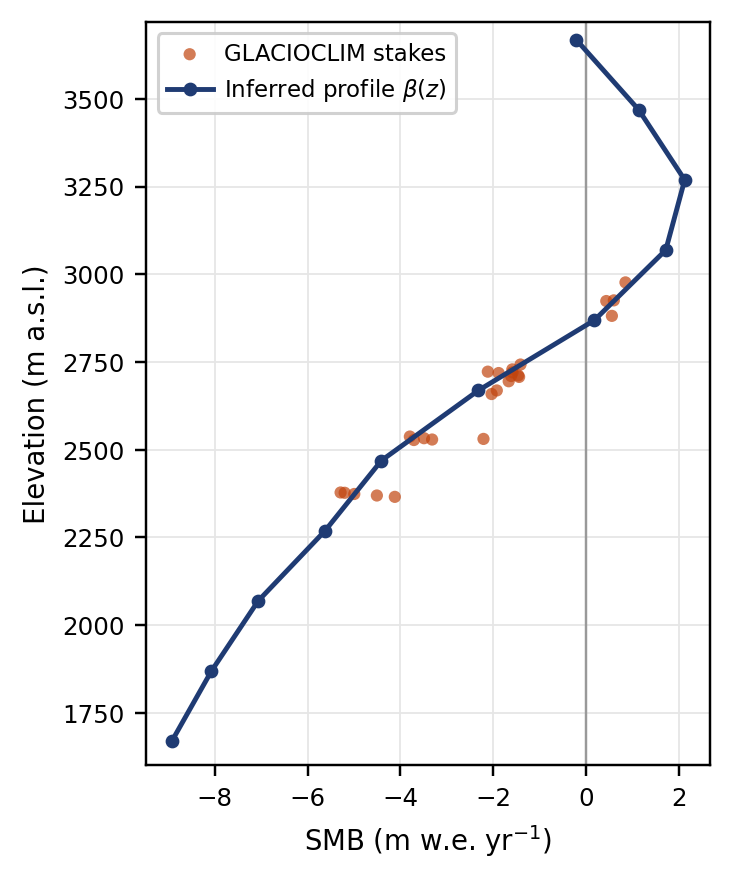
\includegraphics[width=0.7\linewidth]{figs/argentiere_smb_profile.png}
%DIFDELCMD <   %%%
%DIFDELCMD < \caption{%
{%DIFAUXCMD
\DIFdelFL{Inferred elevation-resolved SMB profile $\beta(z)$ (blue) for Argentière
    over 2012--2021 from the GPR-assisted inversion, in water equivalent. Orange dots
    are the 2012--2021 mean GLACIOCLIM stake balances, plotted at the elevation of
    each stake. The profile spans $1670$--$3610\,\mathrm{m\,a.s.l.}$ and matches the
    stakes with $\mathrm{RMSE}=0.45\,\mathrm{m\,w.e.\,yr^{-1}}$.}}
  %DIFAUXCMD
%DIFDELCMD < \label{fig:gpr-smb}
%DIFDELCMD < \end{figure}
%DIFDELCMD < 

%DIFDELCMD < \begin{figure*}
%DIFDELCMD <   \centering
%DIFDELCMD <   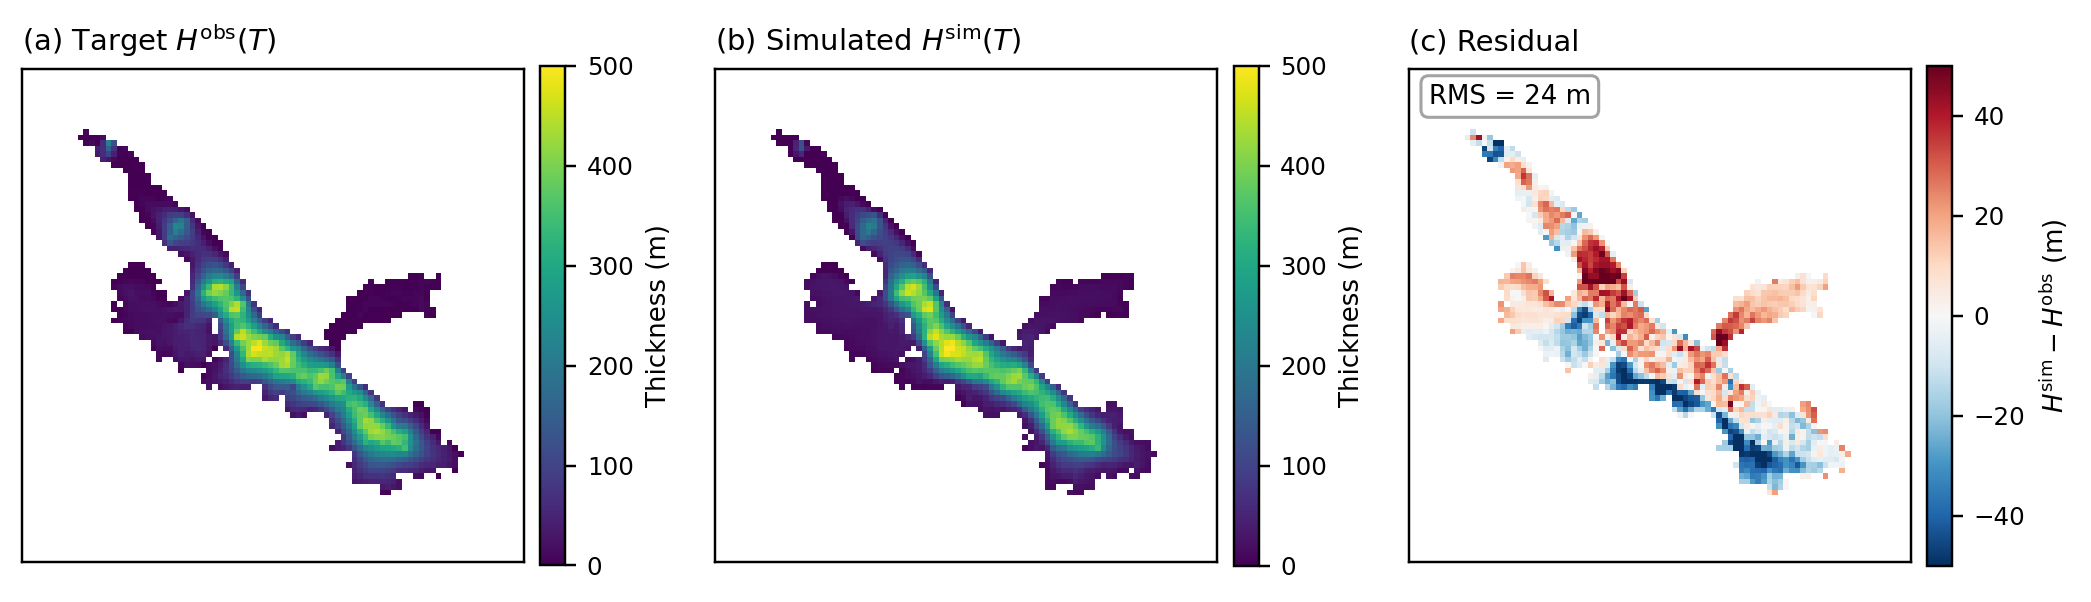
\includegraphics[width=\linewidth]{figs/argentiere_thk_comparison.png}
%DIFDELCMD <   %%%
%DIFDELCMD < \caption{%
{%DIFAUXCMD
\DIFdelFL{End-of-window ice-thickness fit on Argentière ($t_2 = 2021$), masked to
    the glacier footprint. (a)~Target thickness $H^{\mathrm{obs}}(\cdot, t_2)$ from
    the observed surface DEM and the calibrated bedrock; (b)~simulated thickness
    $H^{\mathrm{sim}}(\cdot, t_2)$ from the forward run under the inferred SMB
    profile; (c)~their residual $H^{\mathrm{sim}} - H^{\mathrm{obs}}$
    (RMS $24\,\mathrm{m}$). The residual is small and largely unbiased; its spatially
    structured component reflects horizontal variability within elevation bands that
    the one-dimensional profile does not represent.}}
  %DIFAUXCMD
%DIFDELCMD < \label{fig:gpr-thk}
%DIFDELCMD < \end{figure*}
%DIFDELCMD < 

%DIFDELCMD < %%%
\DIFdelend \subsection{Applicability to near-global elevation-change data}\label{app:hugonnet}

The fidelity of the inferred SMB is ultimately set by the quality of the input
elevation change (Sect.~\ref{sec:contribution}). The main results use dedicated
two-epoch DEMs, which deliver the highest accuracy but are not available everywhere.
Near-global elevation-change products such as that of \citet{hugonnet2021} would, by
contrast, make the method applicable to essentially any glacier. To gauge the
associated fidelity penalty \DIFaddbegin \DIFadd{in isolation}\DIFaddend , we repeat the inversion on
Rhône---chosen for its denser stake \DIFdelbegin \DIFdel{record ($n=5$ continuous-record
locations)---replacing only the geometry-change target: the observed
surface-elevation change is now the \mbox{%DIFAUXCMD
\citet{hugonnet2021} }\hskip0pt%DIFAUXCMD
$\mathrm{d}h/\mathrm{d}t$
rate, while the velocity data assimilation and the }\DIFdelend \DIFaddbegin \DIFadd{record---keeping }\emph{\DIFadd{every}} \DIFadd{other element of
the main-text experiment fixed: the data assimilation is anchored on the same real
swisstopo 2016 DEM (Sect.~\ref{sec:da}), which fixes the same bed; the window is the
same 2007--2016 period; the }\DIFaddend scalar-$\tau_{\mathrm{ref}}$ ensemble search \DIFdelbegin \DIFdel{are left unchanged.
}\DIFdelend \DIFaddbegin \DIFadd{is
unchanged; and validation uses the }\emph{\DIFadd{same}} \DIFadd{$n=5$ 2007--2016 stake set as the
main text. Only the source of the 2007 start-of-window geometry changes: instead of
the surveyed swisstopo 2007 DEM, it is derived as $usurf(2016) -
\dot{h}_{\mathrm{Hugonnet}}\times 9\,\mathrm{yr}$, using \mbox{%DIFAUXCMD
\citet{hugonnet2021}}\hskip0pt%DIFAUXCMD
's mean
2000--2020 rate. Because the two experiments share an identical DA state, this
isolates the effect of the DEM source from that of the validation window. On the
ice-covered area, the Hugonnet-implied 2007 surface differs from the surveyed
swisstopo DEM by a mean of $+3.1\,\mathrm{m}$ (RMS $6.0\,\mathrm{m}$).
}\DIFaddend 

\DIFdelbegin \DIFdel{The }\DIFdelend \DIFaddbegin \DIFadd{Using the same }\DIFaddend velocity-selected coefficient \DIFdelbegin \DIFdel{($\tau_{\mathrm{ref}}=0.12$}\DIFdelend \DIFaddbegin \DIFadd{as the main text
($\tau_{\mathrm{ref}}=0.132$}\DIFaddend \,MPa\DIFdelbegin \DIFdel{, again the surface-velocity-misfit minimum) yields an inferred profile that }\DIFdelend \DIFaddbegin \DIFadd{), the Hugonnet-anchored inversion }\DIFaddend reproduces the
stake averages with a root-mean-square error of \DIFdelbegin \DIFdel{$0.70\,\mathrm{m\,w.e.\,yr^{-1}}$
}\DIFdelend \DIFaddbegin \DIFadd{$0.77\,\mathrm{m\,w.e.\,yr^{-1}}$
}\DIFaddend (Fig.~\ref{fig:hugonnet})---about \DIFdelbegin \DIFdel{twice the $0.32$ }\DIFdelend \DIFaddbegin \DIFadd{$28\,\%$ worse than the $0.60$ }\DIFaddend obtained with the
dedicated swisstopo DEMs \DIFdelbegin \DIFdel{(Sect.~\ref{sec:inferred}}\DIFdelend \DIFaddbegin \DIFadd{at the same $\tau_{\mathrm{ref}}$ and identical validation
window (Table~\ref{tab:hugonnet}}\DIFaddend ), yet still recovering the full altitudinal
structure and remaining well below the stationary-flux continuity estimate
(\DIFdelbegin \DIFdel{$1.79\,\mathrm{m\,w.e.\,yr^{-1}}$}\DIFdelend \DIFaddbegin \DIFadd{$1.56\,\mathrm{m\,w.e.\,yr^{-1}}$, against $1.53$ for the dedicated DEMs at the
same $\tau_{\mathrm{ref}}$}\DIFaddend ). The degradation is concentrated in the \DIFdelbegin \DIFdel{upper ablation and accumulation
area , and reflects }\DIFdelend \DIFaddbegin \DIFadd{accumulation
area (Fig.~\ref{fig:hugonnet}b): the equilibrium-line altitude implied by the
Hugonnet-anchored profile sits $60$--$90\,\mathrm{m}$ higher than its dedicated-DEM
counterpart at every $\tau_{\mathrm{ref}}$ (Table~\ref{tab:hugonnet}), reflecting }\DIFaddend the
stronger spatial smoothing and larger uncertainty of the near-global product
relative to a dedicated DEM pair. This confirms the trade-off anticipated in
Sect.~\ref{sec:contribution}: near-global elevation-change data extend the method to
almost any glacier at a fidelity cost bounded by the DEM quality, so dedicated
multi-temporal DEMs remain preferable where they exist. 


\DIFdelbegin \DIFdel{Exploring the full sliding sweep (Table~\ref{tab:hugonnet}) reinforces this: with the
Hugonnet product the surface-velocity-misfit minimum coincides with the best stake
fit, and the stake error is nearly flat across the whole low-misfit basin
($0.70$--$0.77\,\mathrm{m\,w.e.\,yr^{-1}}$), so the residual sensitivity to
$\tau_{\mathrm{ref}}$ is small next to the fidelity gap between the two
elevation-change sources.
}%DIFDELCMD < 

%DIFDELCMD < %%%
\DIFdelend \begin{table}
  \caption{Sensitivity of the \DIFdelbeginFL \DIFdelFL{Hugonnet-based }\DIFdelendFL Rhône inversion to the basal-motion parameter
    $\tau_{\mathrm{ref}}$ (at \DIFdelbeginFL \DIFdelFL{$A=78$}\DIFdelendFL \DIFaddbeginFL \DIFaddFL{$A=66.8\,\mathrm{MPa^{-3}\,yr^{-1}}$, the main-text
    ensemble-search value}\DIFaddendFL ), \DIFdelbeginFL \DIFdelFL{with }\DIFdelendFL \DIFaddbeginFL \DIFaddFL{comparing }\DIFaddendFL the \DIFaddbeginFL \DIFaddFL{Hugonnet-anchored experiment
    (Hugonnet-implied 2007 surface) against the }\DIFaddendFL dedicated-DEM \DIFdelbeginFL \DIFdelFL{stake RMSE }\DIFdelendFL \DIFaddbeginFL \DIFaddFL{one (surveyed 2007
    surface) }\DIFaddendFL at matching $\tau_{\mathrm{ref}}$\DIFdelbeginFL \DIFdelFL{for comparison}\DIFdelendFL . \DIFaddbeginFL \DIFaddFL{The two experiments share an
    identical DA state (2016 anchor, bed, ensemble search) and are validated
    against the }\emph{\DIFaddFL{same}} \DIFaddFL{$n=5$ 2007--2016 stake set, so the two stake-RMSE
    columns isolate the effect of the 2007 DEM source alone. }\DIFaddendFL \emph{velsurf} is
    \DIFaddbeginFL \DIFaddFL{identical between }\DIFaddendFL the \DIFdelbeginFL \DIFdelFL{surface-velocity misfit and ELA }\DIFdelendFL \DIFaddbeginFL \DIFaddFL{two experiments to }\DIFaddendFL the \DIFdelbeginFL \DIFdelFL{equilibrium-line altitude; }\DIFdelendFL \DIFaddbeginFL \DIFaddFL{precision shown, since }\DIFaddendFL the \DIFdelbeginFL \DIFdelFL{stake RMSE }\DIFdelendFL \DIFaddbeginFL \DIFaddFL{DA
    does not depend on the 2007 surface; ELA }\DIFaddendFL is \DIFaddbeginFL \DIFaddFL{from }\DIFaddendFL the \DIFdelbeginFL \DIFdelFL{validation against }\DIFdelendFL \DIFaddbeginFL \DIFaddFL{Hugonnet experiment (}\DIFaddendFL the
    \DIFdelbeginFL \DIFdelFL{$n=5$ continuous-record averages}\DIFdelendFL \DIFaddbeginFL \DIFaddFL{dedicated-DEM values are $60$--$90\,\mathrm{m}$ lower throughout,
    Fig}\DIFaddendFL .\DIFdelbeginFL \DIFdelFL{Column minima in
    bold}\DIFdelendFL \DIFaddbeginFL \DIFaddFL{~\ref{fig:hugonnet})}\DIFaddendFL . \DIFaddbeginFL \DIFaddFL{Mean improvement: 0.11 m $ w.e. yr^{-1}$, or $~9.8\%$ averaged per-row}\DIFaddendFL }
  \label{tab:hugonnet}
  \centering
  \begin{tabular}{lcccc}
    \toprule
    $\tau_{\mathrm{ref}}$ & velsurf RMSE & ELA \DIFaddbeginFL \DIFaddFL{(Hugonnet) }\DIFaddendFL & \multicolumn{2}{c}{Stake RMSE (m\,w.e.\,yr$^{-1}$)} \\
    (MPa) & (m\,yr$^{-1}$) & (m\,a.s.l.) & Hugonnet & ded.\ DEMs \\
    \midrule
    \DIFdelbeginFL \DIFdelFL{0.121 }\DIFdelendFL \DIFaddbeginFL \DIFaddFL{0.098            }\DIFaddendFL & \textbf{\DIFdelbeginFL \DIFdelFL{7.56}\DIFdelendFL \DIFaddbeginFL \DIFaddFL{7.19}\DIFaddendFL } & \DIFdelbeginFL \DIFdelFL{3136 }\DIFdelendFL \DIFaddbeginFL \DIFaddFL{3041 }\DIFaddendFL & \DIFdelbeginFL \textbf{\DIFdelFL{0.70}} %DIFAUXCMD
\DIFdelendFL \DIFaddbeginFL \DIFaddFL{1.29 }\DIFaddendFL & \DIFdelbeginFL \DIFdelFL{0.81 }\DIFdelendFL \DIFaddbeginFL \DIFaddFL{1.34 }\DIFaddendFL \\
    \DIFdelbeginFL \DIFdelFL{0.154 }\DIFdelendFL \DIFaddbeginFL \DIFaddFL{0.132$^\dagger$  }\DIFaddendFL & \DIFdelbeginFL \DIFdelFL{8.43          }\DIFdelendFL \DIFaddbeginFL \DIFaddFL{7.82          }\DIFaddendFL & \DIFdelbeginFL \DIFdelFL{3096 }\DIFdelendFL \DIFaddbeginFL \DIFaddFL{3116 }\DIFaddendFL & \DIFdelbeginFL \DIFdelFL{0.74 }\DIFdelendFL \DIFaddbeginFL \textbf{\DIFaddFL{0.77}} \DIFaddendFL & \DIFdelbeginFL \DIFdelFL{1.25 }\DIFdelendFL \DIFaddbeginFL \textbf{\DIFaddFL{0.60}} \DIFaddendFL \\
    0.199            & \DIFdelbeginFL \DIFdelFL{9.42          }\DIFdelendFL \DIFaddbeginFL \DIFaddFL{9.45          }\DIFaddendFL & \DIFdelbeginFL \DIFdelFL{3084 }\DIFdelendFL \DIFaddbeginFL \DIFaddFL{3061 }\DIFaddendFL & \DIFdelbeginFL \DIFdelFL{0.77 }\DIFdelendFL \DIFaddbeginFL \DIFaddFL{0.93 }\DIFaddendFL & \DIFdelbeginFL \textbf{\DIFdelFL{0.32}} %DIFAUXCMD
%DIFDELCMD < \\
%DIFDELCMD <     %%%
\DIFdelFL{0.459 }%DIFDELCMD < & %%%
\DIFdelFL{15.35         }%DIFDELCMD < & %%%
\DIFdelFL{3083 }%DIFDELCMD < & %%%
\DIFdelFL{0.73 }%DIFDELCMD < & %%%
\DIFdelendFL 0.77 \\
    0.744            & \DIFdelbeginFL \DIFdelFL{34.77         }\DIFdelendFL \DIFaddbeginFL \DIFaddFL{35.24         }\DIFaddendFL & \DIFdelbeginFL \DIFdelFL{3183 }\DIFdelendFL \DIFaddbeginFL \DIFaddFL{3190 }\DIFaddendFL & \DIFdelbeginFL \DIFdelFL{2.66 }\DIFdelendFL \DIFaddbeginFL \DIFaddFL{2.03 }\DIFaddendFL & \DIFdelbeginFL \DIFdelFL{3.15 }\DIFdelendFL \DIFaddbeginFL \DIFaddFL{1.91 }\DIFaddendFL \\
    1.078            & \DIFdelbeginFL \DIFdelFL{37.43         }\DIFdelendFL \DIFaddbeginFL \DIFaddFL{37.39         }\DIFaddendFL & \DIFdelbeginFL \DIFdelFL{3422 }\DIFdelendFL \DIFaddbeginFL \DIFaddFL{3216 }\DIFaddendFL & \DIFdelbeginFL \DIFdelFL{2.28 }\DIFdelendFL \DIFaddbeginFL \DIFaddFL{1.93 }\DIFaddendFL & \DIFdelbeginFL \DIFdelFL{2.06 }\DIFdelendFL \DIFaddbeginFL \DIFaddFL{1.78 }\DIFaddendFL \\
    \bottomrule
  \end{tabular}
\end{table}

\begin{figure*}
  \centering
  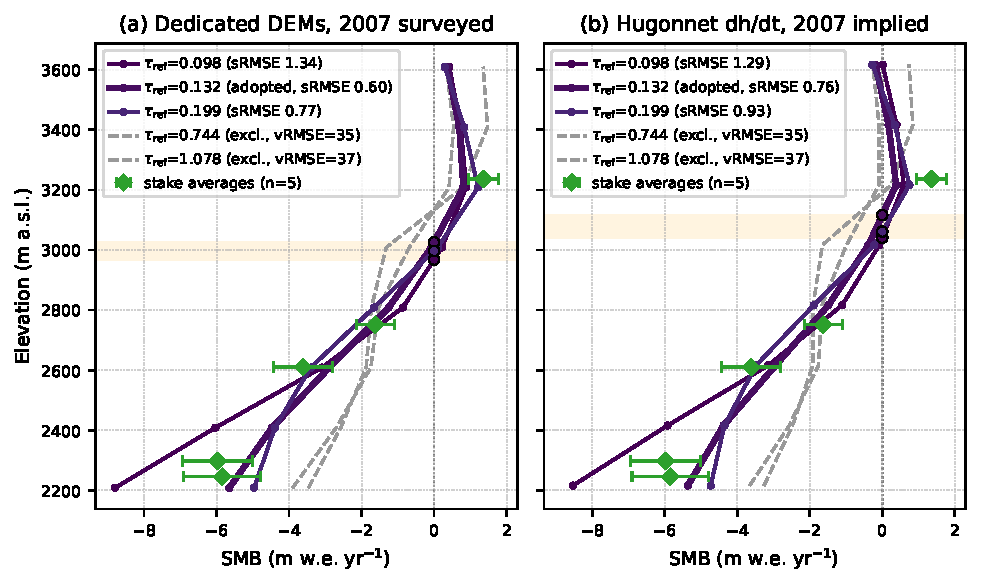
\includegraphics[width=\linewidth]{figs/fig_rhone_sens_2panel.pdf}
  \caption{Sliding-coefficient sensitivity of the Rhône inversion for \DIFdelbeginFL \DIFdelFL{the }\DIFdelendFL two
    \DIFdelbeginFL \DIFdelFL{elevation-change }\DIFdelendFL \DIFaddbeginFL \DIFaddFL{2007--2016 }\DIFaddendFL experiments \DIFaddbeginFL \DIFaddFL{sharing an identical DA state (Sect.~\ref{sec:da},
    anchored on the real 2016 DEM)}\DIFaddendFL : (a)~the \DIFdelbeginFL \DIFdelFL{dedicated two-epoch DEMs }\DIFdelendFL \DIFaddbeginFL \DIFaddFL{surveyed swisstopo 2007 DEM }\DIFaddendFL used in the
    main text and (b)~\DIFaddbeginFL \DIFaddFL{a 2007 surface implied by applying }\DIFaddendFL the \citet{hugonnet2021}
    $\mathrm{d}h/\mathrm{d}t$ product \DIFaddbeginFL \DIFaddFL{backward from the same 2016 DEM}\DIFaddendFL . Each panel
    shows the inferred SMB profile across a range of $\tau_{\mathrm{ref}}$ (colour;
    the \DIFdelbeginFL \DIFdelFL{adopted }\DIFdelendFL profile \DIFaddbeginFL \DIFaddFL{at the main text's adopted $\tau_{\mathrm{ref}}=0.132$ }\DIFaddendFL bold with its
    \DIFdelbeginFL \DIFdelFL{sRMSE}\DIFdelendFL \DIFaddbeginFL \DIFaddFL{stake RMSE}\DIFaddendFL , and runs \DIFdelbeginFL \DIFdelFL{rejected by the
    velocity }\DIFdelendFL \DIFaddbeginFL \DIFaddFL{with velsurf }\DIFaddendFL misfit \DIFaddbeginFL \DIFaddFL{$>1.5\times$ the panel's best rejected,
    }\DIFaddendFL dashed), the equilibrium-line-altitude band shaded \DIFaddbeginFL \DIFaddFL{over the retained runs}\DIFaddendFL , all
    validated against the \DIFdelbeginFL \DIFdelFL{same continuous-record }\DIFdelendFL \DIFaddbeginFL \emph{\DIFaddFL{same}} \DIFaddFL{$n=5$ 2007--2016 }\DIFaddendFL stake averages (green
    diamonds). Both experiments recover the elevation structure, but the
    Hugonnet-based fan sits higher and \DIFdelbeginFL \DIFdelFL{is biased low }\DIFdelendFL \DIFaddbeginFL \DIFaddFL{fits the stakes less well }\DIFaddendFL in the accumulation
    area, giving a larger stake RMSE \DIFaddbeginFL \DIFaddFL{at the adopted $\tau_{\mathrm{ref}}$ }\DIFaddendFL (\DIFdelbeginFL \DIFdelFL{$0.70$ }\DIFdelendFL \DIFaddbeginFL \DIFaddFL{$0.77$ }\DIFaddendFL vs
    \DIFdelbeginFL \DIFdelFL{$0.32\,\mathrm{m\,w.e.\,yr^{-1}}$}\DIFdelendFL \DIFaddbeginFL \DIFaddFL{$0.60\,\mathrm{m\,w.e.\,yr^{-1}}$}\DIFaddendFL ).}
  \label{fig:hugonnet}
\DIFaddbeginFL \end{figure*}

\subsection{\DIFadd{Mechanical equilibrium of the calibrated dynamical state}}\label{app:equilibrium}

\DIFadd{Sect.~\ref{sec:overview} treats the DA-calibrated bedrock, sliding field and
ice-flow emulator as a fixed dynamical substrate and attributes all subsequent
thickness change over the inversion window to the free $smb(z)$ profile
(Sect.~\ref{sec:inference}). That attribution requires the substrate itself to be
close to mechanical equilibrium: if it were not, integrating it forward would
drift even under zero mass-balance forcing, and that drift would alias into the
inferred $smb$ as an initialisation shock \mbox{%DIFAUXCMD
\citep{seroussi2011}}\hskip0pt%DIFAUXCMD
. We test this
directly on Argentière by integrating each of the two candidate starting states
for one year under $smb\equiv 0$ and measuring the resulting on-ice thickness
change: the DA-calibrated state $H_{t_2}$ itself (fit directly to the velocity
observations, Sect.~\ref{sec:da}), and the derived start-epoch state $H_{t_1}$
(Eq.~\ref{eq:hinit}) that the production run actually starts from.
}

\DIFadd{Both states show a near-zero mean drift over the year ($-0.10\,\mathrm{m}$ for
$H_{t_2}$, $-0.33\,\mathrm{m}$ for $H_{t_1}$; Fig.~\ref{fig:shock}c)---an order of
magnitude below the metre-scale annual $smb$ the inversion subsequently
recovers---so neither state is spontaneously gaining or losing mass under the
calibrated dynamics: there is no systematic bias left for the $smb$ inversion to
compensate for. The drift distribution is close to symmetric about zero
(Fig.~\ref{fig:shock}c) and concentrated at a handful of margin and
tributary-confluence cells (Fig.~\ref{fig:shock}a,b) rather than spread evenly
over the glacier, consistent with local relaxation of the discretised stress
balance rather than a large-scale imbalance. In absolute terms this local
redistribution is not negligible---on-ice $\mathrm{RMS}=7.2\,\mathrm{m}$ for
$H_{t_2}$ and $9.7\,\mathrm{m}$ for $H_{t_1}$ (35\,\% larger), against the
$15.8\,\mathrm{m}$ RMS thickness change the $smb$ inversion itself fits over the
full nine-year window (Sect.~\ref{sec:results})---so we report it rather than
discount it; but its near-zero mean and localised footprint show it behaves as
noise the free $smb(z)$ parameters absorb, not as a coherent drift that would bias
the inferred mass balance. 
}

\begin{figure*}
  \centering
  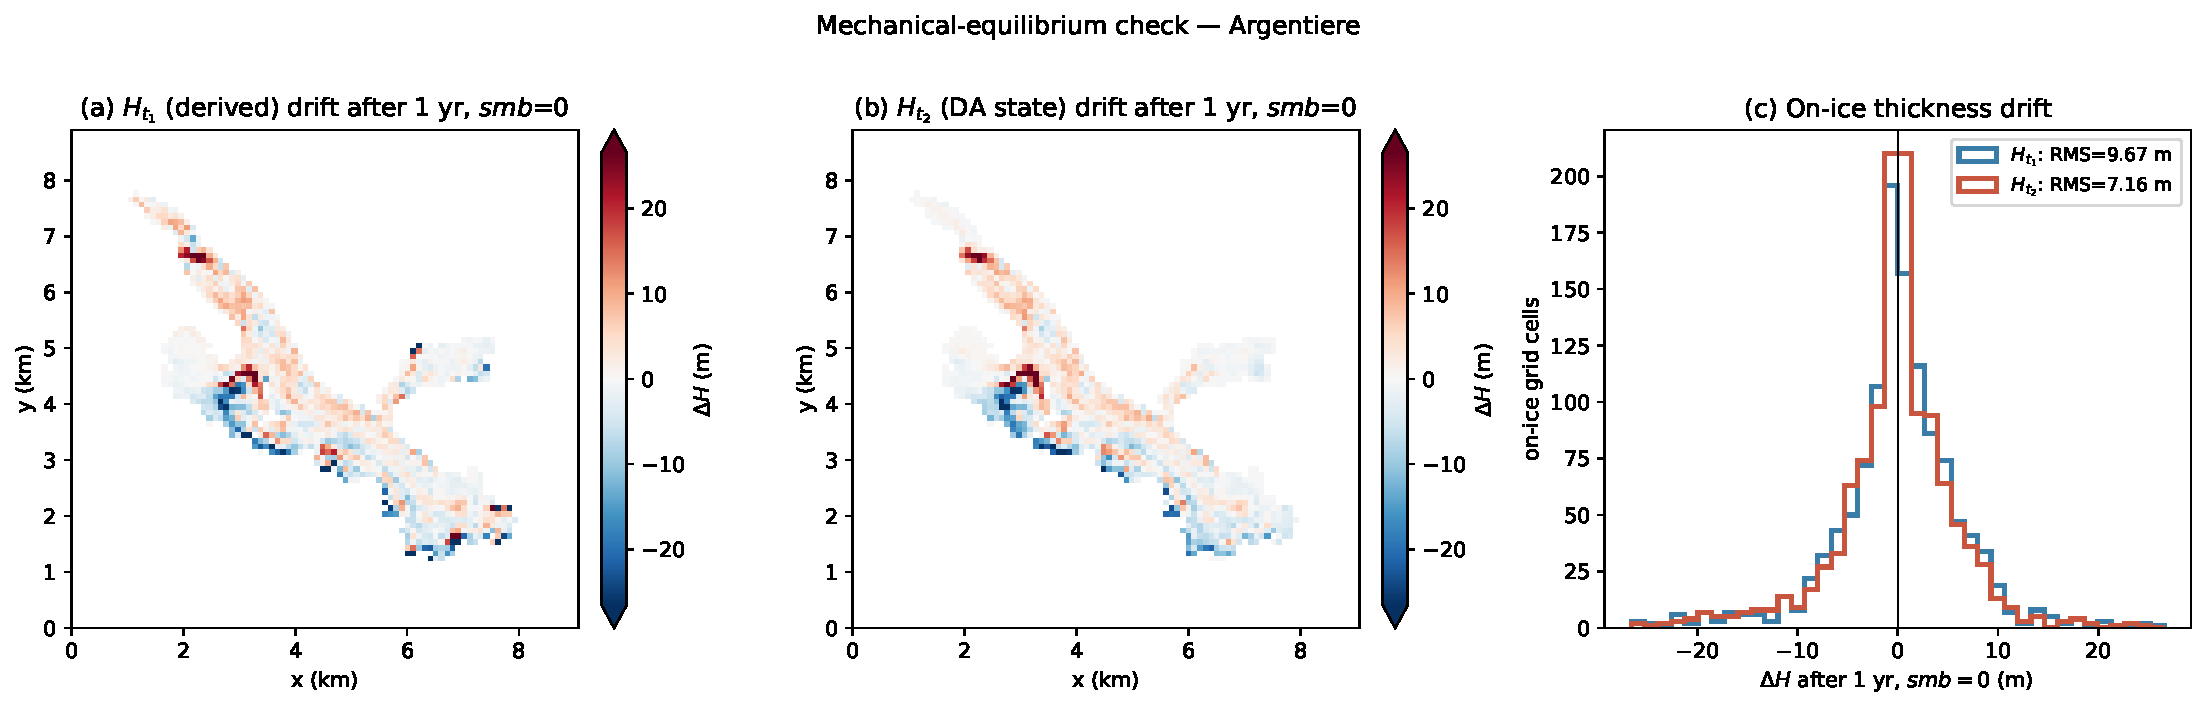
\includegraphics[width=\linewidth]{figs/fig_shock_check.pdf}
  \caption{\DIFaddFL{Mechanical-equilibrium check on Argentière: on-ice thickness drift
    after integrating one year forward under $smb\equiv 0$, starting from (a) the
    derived start-epoch state $H_{t_1}$ and (b) the DA-calibrated state $H_{t_2}$;
    (c) the two drift distributions overlaid, with their on-ice RMS.}}
  \label{fig:shock}
\DIFaddendFL \end{figure*}


\bibliographystyle{copernicus}
\bibliography{\dirbiblio/biblio}

\end{document}
